\section{Cambio de variables}

\begin{definición} [Conjunto Verticalmente Proyectable\label{Conjunto Verticalmente Proyectable}]
Un conjunto $E \subset \mathbb{R}^2$ es verticalmente proyectable si es de la forma:
$$E_1 = \{(x,y) : a \leq x \leq b, f(x) \leq y \leq g(x)\}$$ donde $f,g : [a,b] \to \mathbb{R}$ son funciones continuas con $f(x) \leq g(x)$.
Análogamente se define un conjunto $E \subset \mathbb{R}^2$ es horizontalmente proyectable si es de la forma:
$$E_2 = \{ (x,y) : c \leq y \leq d, \varphi(y) \leq x \leq \psi(y)\}$$
donde $\varphi, \psi : [c,d] \to \mathbb{R}$ son funciones continuas con $\varphi(y) \leq \psi(y)$.
En este caso si $f: E \to \mathbb{R}$ que es integrable en $E$:
$$\int_{E_1}h(x,y)dxdy = \int_{x = a}^{x = b}\left(\int_{y=f(x)}^{y=g(x)}h(x,y)dy\right)dx$$
$$\int_{E_2}h(x,y)dxdy = \int_{y = c}^{y = d}\left(\int_{x=\varphi(y)}^{x=\psi(y)}h(x,y)dx\right)dy$$
\begin{center}
    \begin{minipage}{0.45\textwidth}
        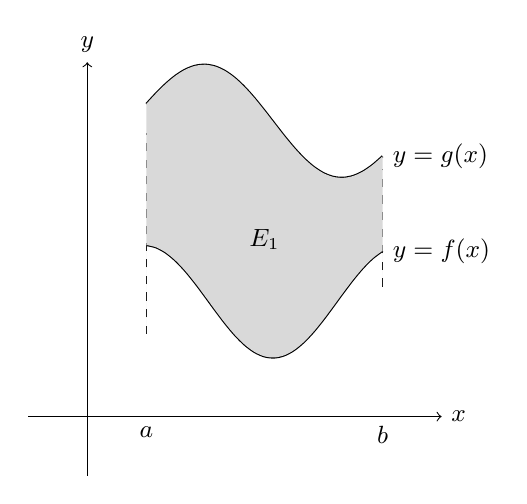
\begin{tikzpicture}[scale=1.5]
            % Ejes
            \draw[->] (-0.5,0) -- (3,0) node[right] {\small $x$};
            \draw[->] (0,-0.5) -- (0,3) node[above] {\small $y$};

            % Curvas más variadas
            \draw[thick, domain=0.5:2.5, smooth, variable=\x] plot ({\x}, {1 + 0.4*sin(3*\x r) + 0.1*cos(2*\x r)}) node[right] {\small $y = f(x)$}; % Ajuste aquí
            \draw[thick, domain=0.5:2.5, smooth, variable=\x] plot ({\x}, {2.5 - 0.3*cos(3*\x r) + 0.2*sin(2*\x r)}) node[right] {\small $y = g(x)$};

            % Líneas verticales en x=a y x=b
            \draw[dashed] (0.5,0.7) -- (0.5,2.4);
            \draw[dashed] (2.5,1.1) -- (2.5,2.1);

            % Etiquetas a y b
            \node[below] at (0.5,0) {\small $a$};
            \node[below] at (2.5,0) {\small $b$};

            % Región sombreada
            \begin{scope}
                \clip (0.5,0.7) -- plot[domain=0.5:2.5, smooth] (\x, {2.5 - 0.3*cos(3*\x r) + 0.2*sin(2*\x r)}) -- (2.5,1.1) -- plot[domain=2.5:0.5, smooth] (\x, {1 + 0.4*sin(3*\x r) + 0.1*cos(2*\x r)}) -- cycle; % Ajuste aquí
                \fill[gray!30] (0,0) rectangle (3,3);
            \end{scope}

            % Etiqueta de la región
            \node at (1.5,1.5) {\small $E_1$};

        \end{tikzpicture}
    \end{minipage}
    \hspace{0.05\textwidth} % Espacio entre las dos figuras
    \begin{minipage}{0.45\textwidth}

        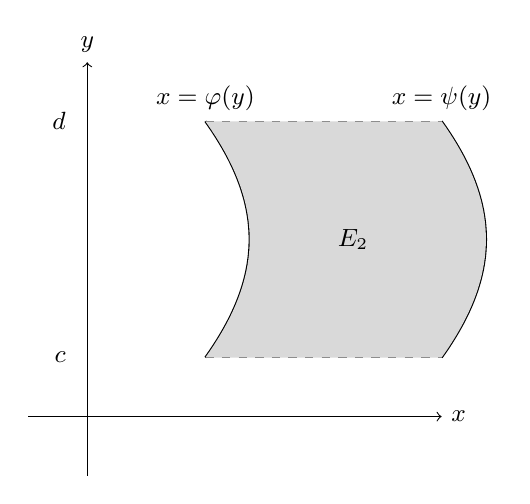
\begin{tikzpicture}[scale=1.5]
            % Ejes de coordenadas con una separación más pequeña
            \draw[->] (-0.5,0) -- (3,0) node[right] {\small $x$};
            \draw[->] (0,-0.5) -- (0,3) node[above] {\small $y$};

            \node[left] at (-0.1,0.5) {\small $c$};  % Etiqueta en y = 0.5
            \node[left] at (-0.1,2.5) {\small $d$};  % Etiqueta en y = 2.5

            % Mover la figura ligeramente a la derecha
            \begin{scope}[shift={(1,0)}]  % Ahora solo 1 unidad a la derecha
                \draw[thick] (0,0.5) .. controls (0.5,1.2) and (0.5,1.8) .. (0,2.5)
                node[above] {\small $x = \varphi(y)$};

                \draw[thick] (2,0.5) .. controls (2.5,1.2) and (2.5,1.8) .. (2,2.5)
                node[above] {\small $x = \psi(y)$};

                % Líneas horizontales
                \draw[dashed] (0,0.5) -- (2,0.5);
                \draw[dashed] (0,2.5) -- (2,2.5);

                % Región sombreada
                \fill[gray!30] (0,0.5) .. controls (0.5,1.2) and (0.5,1.8) .. (0,2.5) --
                (2,2.5) .. controls (2.5,1.8) and (2.5,1.2) .. (2,0.5) -- cycle;

                \node at (1.25,1.5) {\small $E_2$};
            \end{scope}
        \end{tikzpicture}

    \end{minipage}
\end{center}
\end{definición}

\begin{observación}
La diferencia entre ambas definciones es que en la primera se fija $x$ y se mueve $y$ y en la segunda se fija $y$ y se mueve $x$. Lo que tiene como consecuencia que en la primera se integra $dx-dy$ y en la segunda $dy-dx$.
\end{observación}

\begin{teorema}
    Sea $T: \mathbb{R}^n \to \mathbb{R}^n$ aplicación lineal. Sea $A \subset \mathbb{R}^n$ medible $\implies T(A)$ es medible y además:
    \[m(T(A)) = |\det(T)|m(A)\]
\end{teorema}
\begin{definición} [Difeomorfismo\label{difeomorfismo}]
Sean $U, V \subset \mathbb{R}^n$ abiertos se dice que $\varphi: U \to V$ es un difeomorfismo de $U$ a $V$ si:
\vspace{-0.5em}
\begin{enumerate}
    \item $\varphi$ es biyectiva
    \item $\varphi$ es de clase $C^1$ en $U$
    \item $\varphi^{-1}$ es de clase $C^1$ en $V$
\end{enumerate}
\end{definición}
\begin{observación}
Sea $\varphi: U \to \mathbb{R}$ de clase $C^1$ donde $U \subset \mathbb{R}^n$ es abierto, y supongamos que $det(D\varphi(u)) \neq 0 \quad \forall u \in U \implies V = \varphi(U)$ es abierto. Si $\varphi$ es inyectiva, tenemos que $\varphi: U \to \varphi(U) = V$ es un difeomorfismo.
\end{observación}

\begin{teorema}
    Sean $U, V \subset \mathbb{R}^n$ abierto y $\varphi: U \to V$ difeomorfismo-$C^{1}$. Si $A \subset U$ es medible, entonces $\varphi(A)$ es medible y $m(\varphi(A)) = \int_{A}|\det(D\varphi(u))|du$.
\end{teorema}

\begin{teorema}[Teorema del Cambio de Variable\label{TCV}]
    Sean $U,V \subset \mathbb{R}^n$ abiertos y $\varphi: U \to V$ difeomorfismo-$C^1$. Sea $f: V \to \mathbb{R}$ medible. Entonces:
    \begin{enumerate}
        \item Si $f$ es no negativa $\implies (f \circ \varphi) |\det(D\varphi)|$ es medible
              y no-negativa.
        \item Si $f$ es integrable $\implies (f \circ \varphi)|\det(D\varphi)|$ es integrable \end{enumerate}
    En ambos casos se cumple que:
    $$\int_{V = \varphi(U)} f(x)dx = \int_U (f \circ \varphi(u))|\det(D\varphi)|du$$
\end{teorema}
\begin{observación}
Si $A \subset U$ es medible $\implies \varphi(A)$ es medible y
$$\int_{\varphi(A)}f(x)dx = \int_{A}(f \circ \varphi(u))|\det(D\varphi)|du$$
\end{observación}

\ejemplo{
    Sea $\int_{E} e^{\frac{x-y}{x+y}}dxdy$ donde $E = $ tríangulo de vértices $(0,0), (2,0)$ y $(0,2)$.\\
    Si tomamos el cambio de variable: \\ $$\varphi^{-1} \begin{cases} u = x-y \\ v = x+y \end{cases} \implies \varphi \begin{cases} x = \frac{u+v}{2} \\ y = \frac{v - u}{2} \end{cases} \implies f(x,y) = f(u,v) = e^{\frac{u}{v}}$$\\
    Si tomamos la representación gráfica del cambio de variable obtenemos que:
    \begin{center}
    \begin{minipage}{0.45\textwidth}
        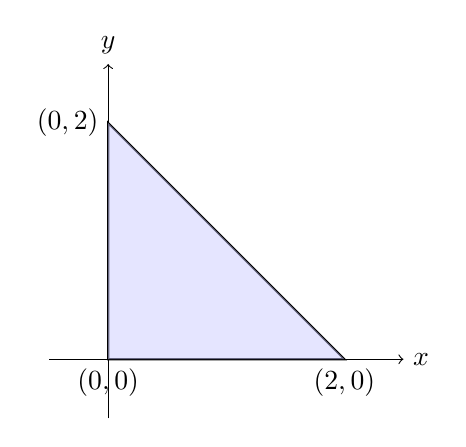
\begin{tikzpicture}[scale=1.5]
            % Ejes coordenados
            \draw[->] (-0.5,0) -- (2.5,0) node[right] {$x$}; % Dibuja el eje x con una flecha en el extremo derecho
            \draw[->] (0,-0.5) -- (0,2.5) node[above] {$y$}; % Dibuja el eje y con una flecha en el extremo superior

            % Triángulo original en xy
            \draw[thick] (0,0) -- (2,0) -- (0,2) -- cycle; % Dibuja el triángulo con vértices en (0,0), (2,0) y (0,2)

            % Etiquetas de los vértices
            \node[below] at (0,0) {$(0,0)$}; % Etiqueta el vértice (0,0)
            \node[below] at (2,0) {$(2,0)$}; % Etiqueta el vértice (2,0)
            \node[left] at (0,2) {$(0,2)$}; % Etiqueta el vértice (0,2)

            % Área sombreada
            \fill[blue!20,opacity=0.5] (0,0) -- (2,0) -- (0,2) -- cycle; % Rellena el triángulo con un color azul claro y opacidad del 50%
        \end{tikzpicture}
    \end{minipage}
    \hspace{0.0000001\textwidth} % Ajusta este valor para cambiar la separación entre las dos minipages
    \begin{minipage}{0.45\textwidth}
        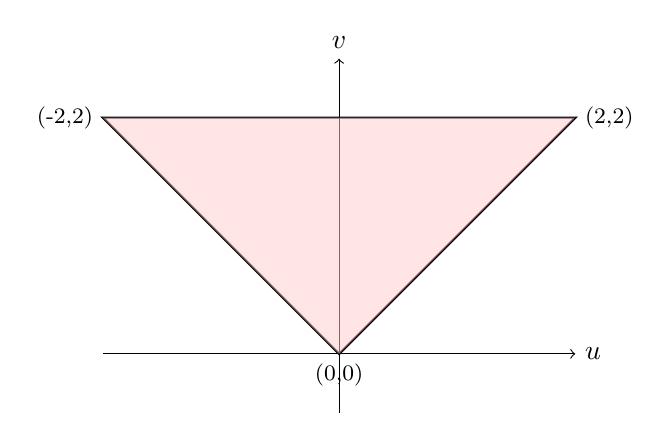
\begin{tikzpicture}[scale=1.5]
            % Ejes coordenados
            \draw[->] (-2,0) -- (2,0) node[right] {$u$};
            \draw[->] (0,-0.5) -- (0,2.5) node[above] {$v$};

            % Triángulo
            \draw[thick] (-2,2) -- (2,2) -- (0,0) -- cycle;

            % Etiquetas de los vértices
            \node[left] at (-2,2) {\footnotesize (-2,2)};
            \node[right] at (2,2) {\footnotesize (2,2)};
            \node[below] at (0,0) {\footnotesize (0,0)};

            \fill[red!20,opacity=0.5] (0,0) -- (2,2) -- (-2,2) -- cycle; % Rellena el triángulo transformado con un color rojo claro y opacidad del 50%
        \end{tikzpicture}
    \end{minipage}
\end{center}

    Si tomamos $y = 0 \implies \varphi^{-1} \begin{cases} u = x \\ v = x \end{cases}$ y también tomamos $x = 0 \implies \begin{cases} u = -y \\ v = y \end{cases}$\\
    en tenemos que $|det(D\varphi)| = \begin{bmatrix} \frac{1}{2} & \frac{1}{2} \\ -\frac{1}{2} & \frac{1}{2} \end{bmatrix} = \frac{1}{2}$\\
    $$\int_{E}f(x,y)dxdy = \int_D e^{\frac{u}{v}} |det(D\varphi)du dv = \int_D \frac{1}{2} e^{\frac{u}{v}}du dv = \frac{1}{2} \int_{v = 0}^{v = 2}\left(\int_{u = -v}^{u = v}e^{\frac{u}{v}}du\right)dv$$
    $$  = \frac{1}{2} \int_{v = 0}^{v = 2}\left[v e^{\frac{u}{v}}\right] _{u = -v}^{u = v} dv = \frac{1}{2} \int_{v = 0}^{v =2}v(e-\frac{1}{e})dv = \frac{1}{2}(e-e^{-1}) \left[\frac{v^2}{2}\right]_{v = 0}^{v=2} = e - e^{-1}$$
}

\subsection{Coordenadas Polares}

\begin{definición}[Coordenadas polares]
En el plano bidimensional $\mathbb{R}^2$, las \textbf{coordenadas polares} $(r, \theta)$ están definidas en términos de las coordenadas cartesianas $(x, y)$ mediante la transformación:

\begin{minipage}{0.5\textwidth}
    \[
        \varphi(r, \theta) =
        \begin{cases}
            x = r\cos\theta, \\
            y = r\sin\theta.
        \end{cases}
    \]
\end{minipage}
\begin{minipage}{0.5\textwidth}
    \centering
    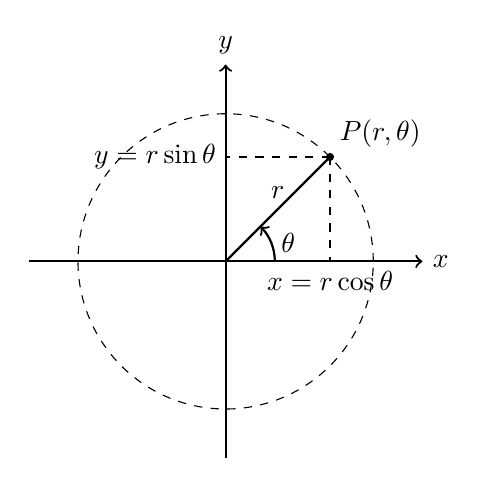
\begin{tikzpicture}[scale=1.25]

    % Draw Cartesian axes
    \draw[->, thick] (-2, 0) -- (2, 0) node[right]{$x$};
    \draw[->, thick] (0, -2) -- (0, 2) node[above]{$y$};

    % Draw a circle to represent the radial distance
    \draw[dashed] (0, 0) circle (1.5);

    % Draw the angle θ
    \draw[->, thick] (0.5, 0) arc (0:45:0.5) node[midway, right]{$\theta$};

    % Draw the radial line
    \draw[thick] (0, 0) -- (45:1.5) node[midway, above]{$r$};

    % Mark the point P(r, θ)
    \filldraw (45:1.5) circle (1pt) node[above right]{$P(r, \theta)$};

    % Draw dashed lines to show projections onto Cartesian axes
    \draw[dashed] (45:1.5) -- ({1.5*cos(45)}, 0) node[below]{$x = r \cos \theta$};
    \draw[dashed] (45:1.5) -- (0, {1.5*sin(45)}) node[left]{$y = r \sin \theta$};

\end{tikzpicture}
\end{minipage}

Donde:
\begin{itemize}
    \item $r \geq 0$ es la distancia radial desde el origen.
    \item $\theta \in [0, 2\pi)$ es el ángulo medido desde el eje positivo $x$ en sentido antihorario.
\end{itemize}

El dominio de la transformación es: $$ U = \{(r, \theta) : r > 0, 0 < \theta <
    2\pi\}. $$ Y su imagen en coordenadas cartesianas es el plano sin el semieje
positivo $x$: $$ V = \mathbb{R}^2 \setminus \{ (x,y) : x \geq 0, y = 0\}. $$

La transformación $\varphi: U \to V$ es un \textbf{difeomorfismo de clase}
$C^1$, ya que cumple las siguientes condiciones:
\begin{itemize}
    \item $\varphi$ es de clase $C^1$, es decir, tiene derivadas continuas en $U$.
    \item $\varphi$ es biyectiva entre $U$ y $V$.
    \item El determinante del Jacobiano es no nulo: $$ \det(D_{\varphi})(r, \theta) = \begin{vmatrix}
                  \frac{\partial x}{\partial r} & \frac{\partial x}{\partial \theta} \\
                  \frac{\partial y}{\partial r} & \frac{\partial y}{\partial \theta}
              \end{vmatrix} =
              \begin{vmatrix}
                  \cos\theta & -r\sin\theta \\
                  \sin\theta & r\cos\theta
              \end{vmatrix} = r\cos^2\theta + r\sin^2\theta = r \neq 0.
          $$
\end{itemize}
Esto implica que el elemento diferencial de área en coordenadas polares es:
$$
    dA = r \, dr \, d\theta.
$$
\end{definición}

\ejemplo{
    \begin{itemize}
        \item Área del círculo $D = \{ (x,y) : x^2 + y^2 \leq R^2\}$ de centro $(0,0)$ y radio $R$:
              $$ \text{Área}(D) = \text{Área}(D \cap V) = \int_{\varphi^{-1}(D \cap V)} f(r \cos\theta, r \sin\theta) \left| \det(D_{\varphi(r, \theta)}) \right| dr d\theta. $$
              Evaluando la integral:
              $$ \int_{\theta=0}^{\theta=2\pi} \left( \int_{r=0}^{r=R} r \, dr \right) d\theta = \pi R^2. $$

        \item Para la región $A = \{(x,y) : x^2 + y^2 \leq 1, \, y \geq 0\}$ con $f(x,y) =
                  \sqrt{x^2+y^2}$: $$ \int_{A} f(x,y) \, dx \, dy = \int_{\theta = 0}^{\theta =
                      \pi} \left( \int_{r = 0}^{r = 1} r \cdot r \, dr \right) d\theta. $$
              Resolviendo: $$ \pi \cdot \int_{r = 0}^{r = 1} r^2 \, dr = \frac{\pi}{3}. $$
    \end{itemize}
}
\ejemplo{
    Realicemos el cálculo de integrales gaussianas:

    \begin{enumerate}
        % Integral gaussiana en una dimensión
        \item $g(t) = e^{-t^2}$: Es fácil ver que $g(t) \geq 0$ es integrable en $\mathbb{R}$. Para ver dicha integral, separemos $\mathbb{R} = (-\infty,0) \cup [0,+\infty)$.

              \begin{enumerate}
                  \item Para $(0, +\infty)$: Si $t \geq 1 \implies t^2 \geq t \implies e^{-t^2} \leq
                            e^{-t}$. Entonces: $$ \int_{t=0}^{t=+\infty} e^{-t^2} dt = \int_{t=0}^{t=1} e^{-t^2}dt
                            + \int_{t=1}^{t=+\infty}e^{-t^2}dt \leq 1 + \int_{t=1}^{t=+\infty}e^{-t^2}dt \leq 1 +
                            e^{-1} < +\infty. $$

                  \item Para $(-\infty, 0)$: Consideremos la integral: $$ \int_{t=-\infty}^{t=0}e^{-t^2}dt$$ 
                  Tomamos el cambio de variable $s = -t$, lo que implica $ds = -dt$. Entonces,
                        la integral se transforma en: $$ \int_{t=-\infty}^{t=0} e^{-s^2} (-ds) =
                            \int_{t=0}^{t=+\infty} e^{-s^2} ds $$ Por lo tanto, $$ \int_{t=-\infty}^{t=0} e^{-t^2}
                            dt = \int_{t=0}^{t=+\infty} e^{-t^2} dt $$ Luego, la integral total es: $$ I =
                            \int_{t=-\infty}^{t=+\infty}e^{-t^2}dt = 2\int_{t=0}^{t=+\infty}e^{-t^2}dt $$
              \end{enumerate}

              % Integral gaussiana en dos dimensiones
        \item Para $f(x,y) = e^{-(x^2+y^2)}$, existen dos maneras de calcular la integral:

              \begin{enumerate}
                  \item Usando coordenadas polares:
                        $$
                            \int_{\mathbb{R}^2}e^{-(x^2+y^2)}dx dy = \int_{\theta=0}^{\theta=2\pi} \left( \int_{r=0}^{r=+\infty}e^{-r^2}r dr \right)d\theta.
                        $$
                        Separando las integrales:
                        $$
                            \left(\int_{\theta=0}^{\theta=2\pi} 1 \, d\theta\right) \left(\int_{r=0}^{r=+\infty} e^{-r^2} r \, dr\right).
                        $$
                        Evaluando la integral en $r$:
                        $$
                            \int_{r=0}^{r=+\infty} e^{-r^2} r \, dr = \left[-\frac{1}{2}e^{-r^2}\right]_{r=0}^{r=+\infty} = \frac{1}{2}.
                        $$
                        Entonces, el resultado final es:
                        $$
                            2\pi \cdot \frac{1}{2} = \pi.
                        $$

                  \item Usando el producto de integrales unidimensionales:
                        $$
                            \int_{x = -\infty}^{x = +\infty}\left(\int_{y = -\infty}^{y = +\infty}e^{-(x^2+y^2)}dy\right)dx.
                        $$
                        Como la exponencial es separable, podemos escribir:
                        $$
                            \int_{x=-\infty}^{x=+\infty} e^{-x^2}dx \cdot \int_{y=-\infty}^{y=+\infty} e^{-y^2}dy.
                        $$
                        Definiendo $I = \int_{-\infty}^{+\infty} e^{-x^2}dx$, se tiene que:
                        $$
                            I^2 = \pi \implies I = \sqrt{\pi}.
                        $$
                        Así, la integral en $\mathbb{R}^2$ es:
                        $$
                            I^2 = \pi.
                        $$
              \end{enumerate}
    \end{enumerate}
}

\ejemplo{
    \underline{Curvas en coordenadas polares}

    Calculemos el área encerrada por la curva en coordenadas polares $$ r = a(1 +
        \cos\theta), $$ la cual describe un cardioide con $a > 0$.

    \textbf{Análisis del comportamiento de $r$:}
    Evaluemos $r$ en algunos valores característicos de $\theta$:

    \[
        \begin{array}{c|c|c}
            \theta         & r = a(1 + \cos\theta) & Comportamiento               \\ \hline
            0              & 2a                    & r \text{ decrece} \downarrow \\
            \frac{\pi}{2}  & a                     & r \text{ decrece} \downarrow \\
            \pi            & 0                     & r \text{ aumenta} \uparrow   \\
            \frac{3\pi}{2} & a                     & r \text{ aumenta} \uparrow   \\
            2\pi           & 2a                    & r \text{ aumenta} \uparrow
        \end{array}
    \]

    \textbf{Cálculo del área encerrada:}
    Utilizamos la fórmula del área en coordenadas polares:

    $$
        A = \int_{\theta = 0}^{\theta = 2\pi} \int_{r = 0}^{r = a(1 + \cos\theta)} r \, dr \, d\theta.
    $$

    Evaluando la integral interna:

    $$
        \int_{r=0}^{r=a(1 + \cos\theta)} r \, dr = \left[ \frac{r^2}{2} \right]_{r=0}^{r=a(1 + \cos\theta)}
        = \frac{a^2}{2} (1 + \cos\theta)^2.
    $$

    Ahora resolvemos la integral en $\theta$:

    $$
        A = \frac{a^2}{2} \int_{\theta=0}^{\theta=2\pi} (1 + 2\cos\theta + \cos^2\theta) \, d\theta.
    $$

    Usando la identidad trigonométrica:

    $$
        \cos^2\theta = \frac{1 + \cos 2\theta}{2},
    $$

    la integral se reescribe como:

    $$
        A = \frac{a^2}{2} \int_{0}^{2\pi} \left( 1 + 2\cos\theta + \frac{1 + \cos 2\theta}{2} \right) d\theta.
    $$

    Evaluamos término a término:

    - $\int_{0}^{2\pi} 1 \, d\theta = 2\pi$.
    - $\int_{0}^{2\pi} \cos\theta \, d\theta = 0$.
    - $\int_{0}^{2\pi} \cos 2\theta \, d\theta = 0$.

    Por lo tanto:

    $$
        A = \frac{a^2}{2} \left( 2\pi + \frac{2\pi}{2} \right) = \frac{3\pi}{2} a^2.
    $$

    \textbf{Conclusión:}
    El área encerrada por el cardioide es:

    $$
        A = \frac{3\pi}{2} a^2.
    $$
}

\subsection{Coordenadas Cilíndricas}

\begin{definición}[Coordenadas cilíndricas]
En el espacio tridimensional, las \textbf{coordenadas cilíndricas} $(r, \theta, z)$ están definidas en términos de las coordenadas cartesianas $(x, y, z)$ mediante la transformación:\\

\begin{minipage}{0.5\textwidth}
    \[
        \varphi(r, \theta, z) =
        \begin{cases}
            x = r\cos\theta, \\
            y = r\sin\theta, \\
            z = z.
        \end{cases}
    \]
\end{minipage}
\begin{minipage}{0.5\textwidth}
    \centering
    %Cylindrical Coordinate
\newcommand{\cylindricalcoordinate}[4]{%
\coordinate (#4) at ({#1*cos(#2)},{#1*sin(#2)},{#3});%
\coordinate (#4xy) at ({#1*cos(#2)},{#1*sin(#2)},0);%
}

%Axis Angles
\tdplotsetmaincoords{70}{110}

%Macros
\pgfmathsetmacro{\rvec}{5}
\pgfmathsetmacro{\thetavec}{45}
\pgfmathsetmacro{\zvec}{4}

\pgfmathsetmacro{\drvec}{1.5}
\pgfmathsetmacro{\dphivec}{20}
\pgfmathsetmacro{\dzvec}{1}

%Layers
\pgfdeclarelayer{background}
\pgfdeclarelayer{foreground}

\pgfsetlayers{background, main, foreground}

\begin{tikzpicture}[tdplot_main_coords, scale=0.75]

%Coordinates
\coordinate (O) at (0,0,0);
%%
\cylindricalcoordinate{\rvec}{\thetavec}{\zvec}{A}
\cylindricalcoordinate{\rvec}{\thetavec}{(\zvec+\dzvec)}{B}
\cylindricalcoordinate{\rvec}{(\thetavec+\dphivec)}{\zvec}{C}
\cylindricalcoordinate{\rvec}{(\thetavec+\dphivec)}{(\zvec+\dzvec)}{D}
%%
\cylindricalcoordinate{(\rvec+\drvec)}{\thetavec}{\zvec}{A'}
\cylindricalcoordinate{(\rvec+\drvec)}{\thetavec}{(\zvec+\dzvec)}{B'}
\cylindricalcoordinate{(\rvec+\drvec)}{(\thetavec+\dphivec)}{\zvec}{C'}
\cylindricalcoordinate{(\rvec+\drvec)}{(\thetavec+\dphivec)}{(\zvec+\dzvec)}{D'}
%%%Nodes
%\node at (A) {A};
%\node at (B) {B};
%\node at (C) {C};
%\node at (D) {D};
%\node at (A') {A'};
%\node at (B') {B'};
%\node at (C') {C'};
%\node at (D') {D'};

%Axis
\begin{pgfonlayer}{background}
	\draw[thick,-latex] (0,0,0) -- (6,0,0) node[pos=1.1]{$x$};
	\draw[thick,-latex] (0,0,0) -- (0,6,0) node[pos=1.05]{$y$};
	\draw[thick,-latex] (0,0,0) -- (0,0,7) node[pos=1.05]{$z$};
\end{pgfonlayer}

%Vectors
\begin{pgfonlayer}{main}
	\draw[blue, thick] (O) -- (A);
	\draw[thick] (O) -- (Axy) node [pos=0.6, below left] {$r$};
	\draw (A) -- ($(A)-(Axy)$) node [left] {$z$};
	\draw (B) -- ($(A)-(Axy)+(0,0,\dzvec)$) node [left] {$z+\mathrm{d}z$};
	\draw (D) -- ($(A)-(Axy)+(0,0,\dzvec)$);
\end{pgfonlayer}
\begin{pgfonlayer}{background}
	\draw[dashed] (C) -- ($(A)-(Axy)$) node [left] {$z$};
\end{pgfonlayer}

%Help Lines
\begin{pgfonlayer}{background}
	\draw (A) -- (Axy);
	\draw (A') -- (A'xy);
	\draw[thick] (Axy) -- (A'xy) node [pos=0.6, below left] {$\mathrm{d}r$};
	%
	\draw (O) -- (D'xy);
	\draw[dashed] (C) -- (Dxy);	
	\draw (C') -- (C'xy);
	%%Arcs
	\tdplotdrawarc{(0,0,0)}{\rvec}{\thetavec}{\thetavec+\dphivec}{}{}
	\tdplotdrawarc{(0,0,0)}{\rvec+\drvec}{\thetavec}{\thetavec+\dphivec}{}{}
\end{pgfonlayer}

%Angles
\begin{pgfonlayer}{foreground}
	%Phi, dPhi
	\tdplotdrawarc[-stealth]{(O)}{0.9}{0}{\thetavec}{anchor=north}{$\theta$}
	\tdplotdrawarc[-stealth]{(O)}{1.5}{\thetavec}{\thetavec + \dphivec}{}{}
	\node at (1.4,1.9,0) {$\mathrm{d}\theta$};	
\end{pgfonlayer}

%Differential Volume

%%Lines
\begin{pgfonlayer}{foreground}
	\draw[thick] (A) -- (B) -- (B') -- (A') -- cycle node [midway, below] {$\mathrm{d}r$};
	\draw[thick] (D) -- (D') -- (C') node [midway, right] {$\mathrm{d}z$};
\end{pgfonlayer}
\begin{pgfonlayer}{background}
	\draw[thick, dashed] (C') -- (C) -- (D);
\end{pgfonlayer}

%%Curved
\begin{pgfonlayer}{background}
	\tdplotdrawarc[thick, dashed]{(0,0,\zvec)}{\rvec} {\thetavec}{\thetavec+\dphivec}{}{}
\end{pgfonlayer}
\begin{pgfonlayer}{foreground}
	\tdplotdrawarc[thick]{(0,0,\zvec+\dzvec)}{\rvec} {\thetavec}{\thetavec+\dphivec}{}{}
	\node at (2.4,3.4,\zvec+\dzvec) {$r\mathrm{d}\theta$};
	\tdplotdrawarc[thick]{(0,0,\zvec+\dzvec)}{\rvec+\drvec} {\thetavec}{\thetavec+\dphivec}{}{}
	\tdplotdrawarc[thick]{(0,0,\zvec)}{\rvec+\drvec} {\thetavec}{\thetavec+\dphivec}{}{}
\end{pgfonlayer}

%%Fill Color
\begin{pgfonlayer}{main}
	%Front
	\fill[black, opacity=0.15] (B) to (B') to[bend right=4] (D') to (D) to[bend left=4] cycle;
	\fill[black, opacity=0.6] (B') to[bend right=4] (D') to (C') to[bend left=4] (A') to cycle;
	\fill[black, opacity=0.4] (B) to (B')  to (A') to (A) to cycle;
\end{pgfonlayer}
\begin{pgfonlayer}{background}
	%Back
	\fill[black!50, opacity=0.5] (D) to (D') to (C') to (C) to cycle;
	\fill[black!50, opacity=0.5] (B) to[bend right=4] (D) to (C) to[bend left=4] (A) to cycle;
	\fill[black!50, opacity=0.5] (A) to (A') to[bend right=4] (C') to (C) to[bend left=4] cycle;
\end{pgfonlayer}


\end{tikzpicture}
\end{minipage}

Donde:
\begin{itemize}
    \item $r \geq 0$ es la distancia radial desde el eje $z$.
    \item $\theta \in [0, 2\pi)$ es el ángulo azimutal, medido desde el eje positivo $x$ en el plano $xy$.
    \item $z \in \mathbb{R}$ representa la coordenada vertical, la misma que en cartesianas.
\end{itemize}

El dominio de la transformación es: $$ U = \{(r, \theta, z) : r > 0, \ 0 <
    \theta \leq 2\pi\}. $$ Y su imagen es el espacio tridimensional excepto el
semieje positivo $x$: $$ V = \mathbb{R}^3 \setminus \{ (x,y,z) : x \geq 0, y =
    0\}. $$

La matriz jacobiana de la transformación es: $$ D\varphi =
    \begin{bmatrix}
        \cos\theta & -r\sin\theta & 0 \\
        \sin\theta & r\cos\theta  & 0 \\
        0          & 0            & 1
    \end{bmatrix}.
$$
Su determinante, que representa el factor de cambio de volumen, es:
$$
    \left| \det(D\varphi) \right| = r > 0.
$$
Esto implica que el elemento diferencial de volumen en coordenadas cilíndricas es:
$$
    dV = r \, dr \, d\theta \, dz.
$$
\end{definición}

\ejemplo{
Sea $V$ el sólido limitado por $z = x^2 + y^2$ y $z = 2$, y consideremos la función:
$$ f(x,y,z) = x^2 + y^2 + z^2$$
Evaluamos la integral:
$$ \int_{V} (x^2 + y^2 + z^2) \, dx \, dy \, dz$$
Cambiamos a coordenadas cilíndricas, donde $x^2 + y^2 = r^2$, obteniendo:
$$ \int_{z = 0}^{z=2} \int_{\theta = 0}^{\theta=2\pi} \int_{r = 0}^{r=\sqrt{z}} (r^2 + z^2) \cdot r \, dr \, d\theta \, dz$$
Separando la integral en términos de $\theta$:
$$ \left( \int_{\theta = 0}^{\theta=2\pi} 1 \, d\theta \right)
    \left( \int_{z = 0}^{z=2} \left( \int_{r = 0}^{r=\sqrt{z}} (r^3 + z^2 r) \, dr \right) dz \right)$$
Resolviendo la integral en $\theta$:
$$ 2\pi \int_{z = 0}^{z=2} \left[ \frac{r^4}{4} + \frac{z^2 r^2}{2} \right]_{r = 0}^{r = \sqrt{z}} dz$$
Sustituyendo $r = \sqrt{z}$:
$$ 2\pi \int_{z = 0}^{z=2} \left( \frac{z^2}{4} + \frac{z^3}{2} \right) dz$$
Resolviendo la integral en $z$:
$$ 2\pi \left[ \frac{z^3}{12} + \frac{z^4}{8} \right]_{z = 0}^{z = 2}$$
Evaluando los límites:
$$ 2\pi \left( \frac{8}{12} + \frac{16}{8} \right) = 2\pi \left( \frac{2}{3} + 2 \right) = 2\pi \left( \frac{8}{3} \right) = \frac{16\pi}{3}$$
Por lo tanto, el resultado final es:
$$ \frac{16\pi}{3}$$
}

\ejemplo{


Sea \( V \) la porción de la semiesfera \( 0 \leq z \leq \sqrt{2 - x^2 -
    y^2} \) que está fuera del cilindro \( x^2 + y^2 = 1 \).\\
Queremos calcular la integral
\[
    I = \int_V z \,dx\,dy\,dz
\]
En coordenadas cilíndricas, las variables se expresan como:
$$ \varphi(r, \theta, z) =
\begin{cases}
    x = r\cos\theta, \\
    y = r\sin\theta, \\
    z = z.
\end{cases}
$$

donde el jacobiano de la transformación es \( r \).
Los límites en estas coordenadas son:

\begin{itemize}
    \item \( 0 \leq z \leq 1 \) porque la semiesfera en z llega hasta \( \sqrt{2 - x^2 - y^2} \), pero solo consideramos de $z=0$ hasta \( z = 1 \), pues los puntos de la esfera donde $1 \leq z \leq \sqrt{2}$ están dentro del cilindro, luego no los consideramos.
    \item \( 1 \leq r \leq \sqrt{2 - z^2} \) porque el cilindro \( x^2 + y^2 = 1 \) define el límite inferior y la semiesfera define el superior.
    \item \( 0 \leq \theta \leq 2\pi \), ya que se recorre toda la circunferencia.
\end{itemize}

Así, la integral se reescribe como:

\[
    I = \int_{\theta=0}^{\theta=2\pi} \int_{z=0}^{z=1} \int_{r=1}^{r=\sqrt{2 - z^2}} z r \, dr \, dz \, d\theta
\]

Calculamos la integral iterada:

\[
    I = \int_{\theta=0}^{\theta=2\pi} \int_{z=0}^{z=1} z \left( \int_{r=1}^{r=\sqrt{2 - z^2}} r \, dr \right) dz \, d\theta
\]

La integral en \( r \) es:

\[
    \int_{r=1}^{r=\sqrt{2 - z^2}} r \, dr = \left[ \frac{r^2}{2} \right]_{r=1}^{r=\sqrt{2 - z^2}} = \frac{(2 - z^2)}{2} - \frac{1}{2} = \frac{1 - z^2}{2}
\]

Sustituyendo en la integral:

\[
    I = \int_{\theta=0}^{\theta=2\pi} \int_{z=0}^{z=1} z \cdot \frac{1 - z^2}{2} \, dz \, d\theta
\]

Resolviendo la integral en \( z \):

\[
    \frac{1}{2} \int_{z=0}^{z=1} z (1 - z^2) \, dz = \frac{1}{2} \int_{z=0}^{z=1} (z - z^3) \, dz
\]

Calculamos:

\[
    \frac{1}{2} \left[ \frac{z^2}{2} - \frac{z^4}{4} \right]_{z=0}^{z=1} = \frac{1}{2} \left( \frac{1}{2} - \frac{1}{4} \right) = \frac{1}{2} \cdot \frac{1}{4} = \frac{1}{8}
\]

Finalmente, integramos en \( \theta \):

\[
    \int_{\theta=0}^{\theta=2\pi} \frac{1}{8} \, d\theta = 2\pi \frac{1}{8}  = \frac{\pi}{4}
\]

Luego, la integral es:

\[
    I = \frac{\pi}{4}
\]
}

\subsection{Coordenadas Esféricas}

\begin{definición}[Coordenadas esféricas]
En el espacio tridimensional, las coordenadas esféricas $(r, \theta, \phi)$ se definen en términos de las coordenadas cartesianas $(x, y, z)$ mediante la transformación:\\

\begin{minipage}{0.5\textwidth}
    \[
        \varphi(r, \theta, \phi) =
        \begin{cases}
            x = r\cos\theta \sin\phi, \\
            y = r\sin\theta \sin\phi, \\
            z = r\cos\phi.
        \end{cases}
    \]
\end{minipage}
\begin{minipage}{0.5\textwidth}
    \centering
        \tdplotsetmaincoords{70}{120}
    %
    \begin{tikzpicture}[tdplot_main_coords]
        % Coordinates of the location of the differential of volume
        \pgfmathsetmacro{\x}{0.75}
        \pgfmathsetmacro{\y}{1.5}
        \pgfmathsetmacro{\z}{2.25}
        \pgfmathsetmacro{\step}{0.025}
        % coordinates in spherical coordinates
        \pgfmathsetmacro{\radio}{sqrt(\x*\x+\y*\y+\z*\z)}
        \pgfmathsetmacro{\zf}{\radio+1.0} % To indicate the end point in the z axis
        \pgfmathsetmacro{\angulot}{atan(\y/\x)} % angle $\theta$
        \pgfmathsetmacro{\dominio}{\angulot*pi/180}	% Convert $\theta$ into radians
        \pgfmathsetmacro{\angulop}{acos(\z/\radio)} % angle $\phi$
        \pgfmathsetmacro{\dominiop}{\angulop*pi/180}	% Convert $\phi$ into radians
        % Diferencial
        \pgfmathsetmacro{\dradio}{0.75}	% Differential of $r$
        \pgfmathsetmacro{\dangulot}{10}	% Differential of $\theta$
        \pgfmathsetmacro{\dangulop}{10}	% Differential of $\phi$
        \pgfmathsetmacro{\dominiof}{(\angulot+\dangulot)*pi/180}
        % Vertices of the differential of area 
        % on the xy plane (in polar coordinates)
        \pgfmathsetmacro{\Ax}{\radio*cos(\angulot)}
        \pgfmathsetmacro{\Ay}{\radio*sin(\angulot)}
        \pgfmathsetmacro{\Bx}{(\radio+\dradio)*cos(\angulot)}
        \pgfmathsetmacro{\By}{(\radio+\dradio)*sin(\angulot)}
        \pgfmathsetmacro{\Cx}{(\radio+\dradio)*cos(\angulot+\dangulot)}
        \pgfmathsetmacro{\Cy}{(\radio+\dradio)*sin(\angulot+\dangulot)}
        \pgfmathsetmacro{\Dx}{(\radio)*cos(\angulot+\dangulot)}
        \pgfmathsetmacro{\Dy}{(\radio)*sin(\angulot+\dangulot)}
        % 
        \pgfmathsetmacro{\radiof}{\radio+\dradio}
        \pgfmathsetmacro{\radiorayo}{\radiof+2.0*\dradio}
        \pgfmathsetmacro{\angulotf}{\angulot+\dangulot}
        \pgfmathsetmacro{\angulopf}{\angulop+\dangulop}
        % Location of the node to indicate the angles $\theta$ and $\phi$
        \pgfmathsetmacro{\xnodo}{0.35*cos(0.5*\angulot)}
        \pgfmathsetmacro{\ynodo}{0.35*sin(0.5*\angulot)}
        \pgfmathsetmacro{\xnodop}{0.35*sin(0.5*\angulop)*cos(\angulot)}
        \pgfmathsetmacro{\ynodop}{0.35*sin(\angulop)*sin(\angulot)}
        \pgfmathsetmacro{\znodop}{0.35*cos(0.5*\angulop)}
        \pgfmathsetmacro{\xnododp}{0.85*\radio*sin(0.5*(\angulop+\angulopf))*cos(\angulot)}
        \pgfmathsetmacro{\ynododp}{0.85*\radio*sin(0.5*(\angulop+\angulopf))*sin(\angulot)}
        \pgfmathsetmacro{\znododp}{0.85*\radio*cos(0.5*(\angulop+\angulopf))}
        %
        \pgfmathsetmacro{\xfrayouno}{(\radiof+0.5)*cos(\angulot)}
        \pgfmathsetmacro{\yfrayouno}{(\radiof+0.5)*sin(\angulot)}
        \pgfmathsetmacro{\xfrayodos}{(\radiof+0.5)*cos(\angulotf)}
        \pgfmathsetmacro{\yfrayodos}{(\radiof+0.5)*sin(\angulotf)}
        % Vertices of the differential of area in spherical coordinates
        \pgfmathsetmacro{\Px}{\radio*sin(\angulopf)*cos(\angulot)}
        \pgfmathsetmacro{\Py}{\radio*sin(\angulopf)*sin(\angulot)}
        \pgfmathsetmacro{\Pz}{\radio*cos(\angulopf)}
        \pgfmathsetmacro{\Qx}{\radiof*sin(\angulopf)*cos(\angulot)}
        \pgfmathsetmacro{\Qy}{\radiof*sin(\angulopf)*sin(\angulot)}
        \pgfmathsetmacro{\Qz}{\radiof*cos(\angulopf)}
        \pgfmathsetmacro{\Rx}{\radiof*sin(\angulop)*cos(\angulot)}
        \pgfmathsetmacro{\Ry}{\radiof*sin(\angulop)*sin(\angulot)}
        \pgfmathsetmacro{\Rz}{\radiof*cos(\angulop)}
        \pgfmathsetmacro{\Sx}{\radio*sin(\angulop)*cos(\angulot)}
        \pgfmathsetmacro{\Sy}{\radio*sin(\angulop)*sin(\angulot)}
        \pgfmathsetmacro{\Sz}{\radio*cos(\angulop)}
        % 
        \pgfmathsetmacro{\Tx}{\radio*sin(\angulopf)*cos(\angulotf)}
        \pgfmathsetmacro{\Ty}{\radio*sin(\angulopf)*sin(\angulotf)}
        \pgfmathsetmacro{\Tz}{\radio*cos(\angulopf)}
        \pgfmathsetmacro{\Ux}{\radiof*sin(\angulopf)*cos(\angulotf)}
        \pgfmathsetmacro{\Uy}{\radiof*sin(\angulopf)*sin(\angulotf)}
        \pgfmathsetmacro{\Uz}{\radiof*cos(\angulopf)}
        \pgfmathsetmacro{\Vx}{\radiof*sin(\angulop)*cos(\angulotf)}
        \pgfmathsetmacro{\Vy}{\radiof*sin(\angulop)*sin(\angulotf)}
        \pgfmathsetmacro{\Vz}{\radiof*cos(\angulop)}
        \pgfmathsetmacro{\Wx}{\radio*sin(\angulop)*cos(\angulotf)}
        \pgfmathsetmacro{\Wy}{\radio*sin(\angulop)*sin(\angulotf)}
        \pgfmathsetmacro{\Wz}{\radio*cos(\angulop)}	
        % Points to draw the angle $\phi$
        \pgfmathsetmacro{\Qex}{\radiorayo*sin(\angulopf)*cos(\angulot)}
        \pgfmathsetmacro{\Qey}{\radiorayo*sin(\angulopf)*sin(\angulot)}
        \pgfmathsetmacro{\Qez}{\radiorayo*cos(\angulopf)}
        \pgfmathsetmacro{\Rex}{\radiorayo*sin(\angulop)*cos(\angulot)}
        \pgfmathsetmacro{\Rey}{\radiorayo*sin(\angulop)*sin(\angulot)}
        \pgfmathsetmacro{\Rez}{\radiorayo*cos(\angulop)}
        \pgfmathsetmacro{\Uex}{\radiorayo*sin(\angulopf)*cos(\angulotf)}
        \pgfmathsetmacro{\Uey}{\radiorayo*sin(\angulopf)*sin(\angulotf)}
        \pgfmathsetmacro{\Uez}{\radiorayo*cos(\angulopf)}
        \pgfmathsetmacro{\Vex}{\radiorayo*sin(\angulop)*cos(\angulotf)}
        \pgfmathsetmacro{\Vey}{\radiorayo*sin(\angulop)*sin(\angulotf)}
        \pgfmathsetmacro{\Vez}{\radiorayo*cos(\angulop)}
        % The origin
        \coordinate (O) at (0,0,0);	
        % Coordinate axis
        \draw[thick,->] (0,0,0) -- (\radiof+0.5,0,0) node [below left] {$x$};
        \draw[thick,->] (0,0,0) -- (0,\radiof+0.5,0) node [right] {$y$};
        \draw[thick,->] (0,0,0) -- (0,0,\zf+0.5) node [above] {$z$};
        % Intersection of the sphere of radius $r$ with the plane $y = 0$
        \draw[blue,dashed] plot[domain=0:0.5*pi,smooth,variable=\t] ({\radio*sin(\t r)},{0.0},{\radio*cos(\t r)});
        % Intersection of the sphere of radius $r + dr$ with the plane $y = 0$
        \draw[blue,dashed] plot[domain=0:0.5*pi,smooth,variable=\t] ({\radiof*sin(\t r)},{0.0},{\radiof*cos(\t r)});
        % Differential of area in polar coordinates (on the xy-plane)
        \draw[blue,dashed](0,0,0) --  (\xfrayouno,\yfrayouno,0) node[below left] {$\theta$};	
        \draw[blue,dashed](0,0,0) --  (\xfrayodos,\yfrayodos,0) node [below right] {$\theta + d\theta$};
        % Indication of the angle $\theta$
        \draw[blue] plot[domain=0:\dominio,smooth,variable=\t] ({0.5*cos(\t r)},{0.5*sin(\t r)},{0.0});  % 0.5236
        \node[blue,below] at (\xnodo,\ynodo,0) {$\theta$};		
        %
        \draw[blue,dashed] plot[domain=0:0.5*pi,variable=\t] ({\radio*cos(\t r)},{\radio*sin(\t r)},0.0);
        \node[blue,above left] at (\radio,0,0) {$r$};
        \draw[blue,dashed] plot[domain=0:0.5*pi,variable=\t] ({\radiof*cos(\t r)},{\radiof*sin(\t r)},0.0);
        \node[blue,above left] at (\radiof,0,0) {$r + dr$};
        % Differerential of area
        \draw[blue] (\Ax,\Ay,0) -- (\Bx,\By,0) 
                        -- plot[domain=\dominio:\dominiof,variable=\t] ({\radiof*cos(\t r)},{\radiof*sin(\t r)},0.0)
                        -- (\Dx,\Dy,0) 
                        -- plot[domain=\dominiof:\dominio,smooth,variable=\t] ({\radio*cos(\t r)},{\radio*sin(\t r)},0.0)
                        -- (\Ax,\Ay,0);	
        % Plane at $\theta + d\theta$ (inside of the sphere)
        \draw[blue,dashed,fill=yellow!50,opacity=0.35] 
                (0,0,0) -- (\Dx,\Dy,0) -- plot[domain=0.5*pi:0.0,smooth,variable=\t] 
                    ({\radio*sin(\t r)*cos(\angulotf)},{\radio*sin(\t r)*sin(\angulotf)},{\radio*cos(\t r)}) 
                -- (0,0,0);	
        % lines from the origin to the differential of volume
        \draw[blue,dashed] (O) -- (\Tx,\Ty,\Tz);
        \draw[blue,dashed] (O) -- (\Wx,\Wy,\Wz);
        % Plane at $\theta$ (inside the sphere)
        \draw[blue,dashed,fill=yellow!50,opacity=0.35] 
                (0,0,0) -- (\Ax,\Ay,0) -- plot[domain=0.5*pi:0.0,smooth,variable=\t] 
                    ({\radio*sin(\t r)*cos(\angulot)},{\radio*sin(\t r)*sin(\angulot)},{\radio*cos(\t r)}) 
                -- (0,0,0);	
        % lines from the origin to the differential of volume
        \draw[blue,dashed] (O) -- (\Px,\Py,\Pz);
        \draw[blue,dashed] (O) -- (\Sx,\Sy,\Sz);
        % Arc to indicate the angle $\phi$ 
        \draw[blue] plot[domain=0:\dominiop,smooth,variable=\t] ({0.5*sin(\t r)*cos(\angulot)},{0.5*sin(\t r)*sin(\angulot)},{0.5*cos(\t r)});
        \node[blue,above] at (\xnodop,\ynodop,\znodop) {$\phi$};
        \node[blue] at (\xnododp,\ynododp,\znododp) {$d\phi$};
        % Intersection of the sphere of radius $r$ with the plane $x = 0$
        \draw[blue,dashed] plot[domain=0:0.5*pi,smooth,variable=\t] ({0.0},{\radio*sin(\t r)},{\radio*cos(\t r)});
        % Intersection of the sphere of radius $r + dr$ with the plane $x = 0$
        \draw[blue,dashed] plot[domain=0:0.5*pi,smooth,variable=\t] ({0.0},{\radiof*sin(\t r)},{\radiof*cos(\t r)});
        % Sphere of radius $r$
        \foreach \altura in {0,\step,...,\radio}{
            \pgfmathsetmacro{\r}{sqrt((\radio)^2-(\altura)^2)}
            \draw[cyan,line width=3pt,opacity=0.05] plot[domain=0:0.5*pi,smooth,variable=\t] ({\r*cos(\t r)},{\r*sin(\t r)},{\altura});
            \draw[cyan,thin,opacity=0.25] plot[domain=0:0.5*pi,smooth,variable=\t] ({\r*cos(\t r)},{\r*sin(\t r)},{\altura});
        }
        % The differential of volume in spherical coordinates
        \draw[red,thick] (\Px,\Py,\Pz) -- (\Qx,\Qy,\Qz) -- (\Rx,\Ry,\Rz) -- (\Sx,\Sy,\Sz) -- (\Px,\Py,\Pz);
        \draw[red,thick] (\Tx,\Ty,\Tz) -- (\Ux,\Uy,\Uz) -- (\Vx,\Vy,\Vz) -- (\Wx,\Wy,\Wz) -- (\Tx,\Ty,\Tz);
        \draw[red,thick] (\Px,\Py,\Pz) -- (\Tx,\Ty,\Tz);
        \draw[red,thick] (\Qx,\Qy,\Qz) -- (\Ux,\Uy,\Uz);
        \draw[red,thick] (\Rx,\Ry,\Rz) -- (\Vx,\Vy,\Vz);
        \draw[red,thick] (\Sx,\Sy,\Sz) -- (\Wx,\Wy,\Wz);
        % Sphere of radius $r + dr$
        \foreach \altura in {0,\step,...,\radiof}{
            \pgfmathsetmacro{\r}{sqrt((\radiof)^2-(\altura)^2)}
            \draw[cyan,line width=3pt,opacity=0.05] plot[domain=0:0.5*pi,smooth,variable=\t] ({\r*cos(\t r)},{\r*sin(\t r)},{\altura});
            \draw[cyan,thin,opacity=0.25] plot[domain=0:0.5*pi,smooth,variable=\t] ({\r*cos(\t r)},{\r*sin(\t r)},{\altura});
        }
        % Plane at $\theta + d\theta$ (part that is out of the sphere)
        \draw[blue,dashed,fill=yellow!50,opacity=0.35] 
                (\Cx,\Cy,0) -- (\xfrayodos,\yfrayodos,0) -- plot[domain=0.5*pi:0.0,smooth,variable=\t] 
                    ({\radiof*sin(\t r)*cos(\angulotf)},{\radiof*sin(\t r)*sin(\angulotf)},{\radiof*cos(\t r)}) 
                -- (0,0,\zf) -- (\xfrayodos,\yfrayodos,\zf) -- (\xfrayodos,\yfrayodos,0) -- (\Cx,\Cy,0);	
        % Indication for the angle $\phi$
        \draw[blue,dashed] (\Ux,\Uy,\Uz) -- (\Uex,\Uey,\Uez);
        \draw[blue,dashed] (\Vx,\Vy,\Vz) -- (\Vex,\Vey,\Vez);
        % Plane at $\theta$ (part that is out of the sphere)
        \draw[blue,dashed,fill=yellow!50,opacity=0.35] 
                (\Bx,\By,0) -- (\xfrayouno,\yfrayouno,0) -- plot[domain=0.5*pi:0.0,smooth,variable=\t] 
                    ({\radiof*sin(\t r)*cos(\angulot)},{\radiof*sin(\t r)*sin(\angulot)},{\radiof*cos(\t r)}) 
                -- (0,0,\zf) -- (\xfrayouno,\yfrayouno,\zf) -- (\xfrayouno,\yfrayouno,0) -- (\Bx,\By,0);	
        % Indication for the angle $\phi$
        \draw[blue,dashed] (\Qx,\Qy,\Qz) -- (\Qex,\Qey,\Qez);
        \draw[blue,dashed] (\Rx,\Ry,\Rz) -- (\Rex,\Rey,\Rez);
        %
        % Nodes indicating lengths in the differential of volume
        %
        \pgfmathsetmacro{\SWmx}{0.5*(\Sx+\Wx)}
        \pgfmathsetmacro{\SWmy}{0.5*(\Sy+\Wy)}
        \pgfmathsetmacro{\SWmz}{0.5*(\Sz+\Wz)}
        \draw[<-,shift={(\SWmx,\SWmy,\SWmz)}] (0,0,0) -- (-0.5,-0.5,1.75) node [above] {\footnotesize$r\,\sin\phi\,d\theta$};
        \pgfmathsetmacro{\TWmx}{0.5*(\Wx+\Tx)}
        \pgfmathsetmacro{\TWmy}{0.5*(\Wy+\Ty)}
        \pgfmathsetmacro{\TWmz}{0.5*(\Wz+\Tz)}
        \draw[<-,shift={(\TWmx,\TWmy,\TWmz)}] (0,0,0) -- (-1,0.75,1.5) node [above] {~~~\footnotesize$r\,d\phi$};	
    \end{tikzpicture}

\end{minipage}

Donde:
\begin{itemize}
    \item $r \geq 0$ es la distancia radial desde el origen.
    \item $\theta \in [0, 2\pi)$ es el ángulo azimutal medido en el plano $xy$ desde el eje positivo $x$.
    \item $\phi \in [0, \pi]$ es el ángulo polar o colatitud, medido desde el eje positivo $z$.
\end{itemize}

La matriz jacobiana de esta transformación es: $$ D_\varphi =
    \begin{bmatrix}
        \cos\theta \sin\phi & -r\sin\theta \sin\phi & r\cos\theta \cos\phi \\
        \sin\theta \sin\phi & r\cos\theta \sin\phi  & r\sin\theta \cos\phi \\
        \cos\phi            & 0                     & -r\sin\phi
    \end{bmatrix}.
$$
Su determinante, que representa el factor de cambio de volumen, es:
$$
    \left| \det D_\varphi \right| = r^2 \sin\phi.
$$
Esto implica que el elemento diferencial de volumen en coordenadas esféricas es:
$$
    dV = r^2 \sin\phi \, dr \, d\theta \, d\phi.
$$
\end{definición}
\ejemplo{
    $B_r = \{(x,y,z) : x^2 + y^2 + z^2 \leq R^2\} \implies$ \\ $$vol(B_r) = \int_{B_r}1dxdydz = \int_{\theta=0}^{\theta=2\pi}\left(\int_{\phi=0}^{\phi=\pi}\left(\int_{r=0}^{r=R}r^2\sin(\phi)dr\right)d\phi\right)d\theta = \frac{4}{3}\pi R^3$$
}

\subsection{Coordenadas Elípticas}

\begin{definición}[Coordenadas elípticas]
En el plano, las coordenadas elípticas $(r, \theta)$ se definen en términos de las coordenadas cartesianas $(x, y)$ mediante la transformación:
$$
    \varphi (r, \theta) =
    \begin{cases}
        x = a r \cos\theta, \\
        y = b r \sin\theta.
    \end{cases}
$$
Donde:
\begin{itemize}
    \item $r \geq 0$ es la coordenada radial, que describe la escala de la elipse.
    \item $\theta \in [0, 2\pi)$ es el ángulo que mide la posición en la elipse, similar al ángulo en coordenadas polares.
    \item $a, b > 0$ son constantes que determinan los semiejes de las elipses.
\end{itemize}

La matriz jacobiana de esta transformación es: $$ D_\varphi =
    \begin{bmatrix}
        a\cos\theta & -a r \sin\theta \\
        b\sin\theta & b r \cos\theta
    \end{bmatrix}.
$$

Su determinante, que representa el factor de cambio de área, es: $$ \left| \det
    D_\varphi \right| = a b r. $$

Esto implica que el elemento diferencial de área en coordenadas elípticas es:
$$ dA = a b r \, dr \, d\theta. $$

\end{definición}

\ejemplo{
    Consideremos la región elíptica definida en coordenadas cartesianas como:
    $$
        E = \left\{ (x,y) \mid \frac{x^2}{a^2} + \frac{y^2}{b^2} \leq 1 \right\}.
    $$
    En coordenadas elípticas, esto equivale a:
    $$
        E = \left\{ (r, \theta) \mid 0 \leq \theta \leq 2\pi, 0 \leq r \leq 1 \right\}.
    $$

    \textbf{Cálculo del jacobiano:}
    La matriz jacobiana de la transformación es:
    $$
        D\varphi =
        \begin{bmatrix}
            a\cos\theta & -ar\sin\theta \\
            b\sin\theta & br\cos\theta
        \end{bmatrix}.
    $$
    Su determinante es:
    $$
        \det(D\varphi) = ab r.
    $$

    \textbf{Cálculo del área de la elipse:}
    La integral de área en coordenadas elípticas se expresa como:
    $$
        \text{Área}(E) = \int_{\theta = 0}^{\theta = 2\pi} \int_{r = 0}^{r=1} ab r \, dr \, d\theta.
    $$
    Resolviendo la integral en $r$:
    $$
        \int_{r=0}^{r=1} ab r \, dr = ab \left[\frac{r^2}{2} \right]_{r=0}^{r=1} = \frac{ab}{2}.
    $$
    Evaluando la integral en $\theta$:
    $$
        \int_{\theta = 0}^{\theta = 2\pi} d\theta = 2\pi.
    $$
    Por lo tanto, el área de la elipse es:
    $$
        \text{Área}(E) = 2\pi \cdot \frac{ab}{2} = \pi ab.
    $$

    Así, hemos obtenido el área de la elipse usando coordenadas elípticas. }

\ejemplo{
    Volumen comprendido entre los paraboloides:
    $$ 2z = 4 + \frac{x^2}{3} + y^2, \quad 2z = \frac{2x^2}{3} + 3y^2 $$

    Eliminando $z$: $$ 4 + \frac{x^2}{3} + y^2 = \frac{2x^2}{3} + 3y^2 \iff
        \frac{x^2}{3} + 2y^2 = 4 $$ Lo cual es un cilindro elíptico de $\mathbb{R}^3$.

    Definimos el dominio: $$ E = \left\{ (x,y) \mid \frac{x^2}{3} + 2y^2 \leq 4
        \right\} $$ Luego, el volumen está dado por: $$ \text{vol} = \int_{E} \left(2 +
        \frac{x^2}{6} + \frac{y^2}{2} \right) - \left(\frac{x^2}{3} + \frac{3y^2}{2}
        \right) dx \, dy = \int_{E} \left(2 - \frac{x^2}{6} - y^2 \right) dx \, dy $$

    \vspace{-2.1em}

    \begin{center}
        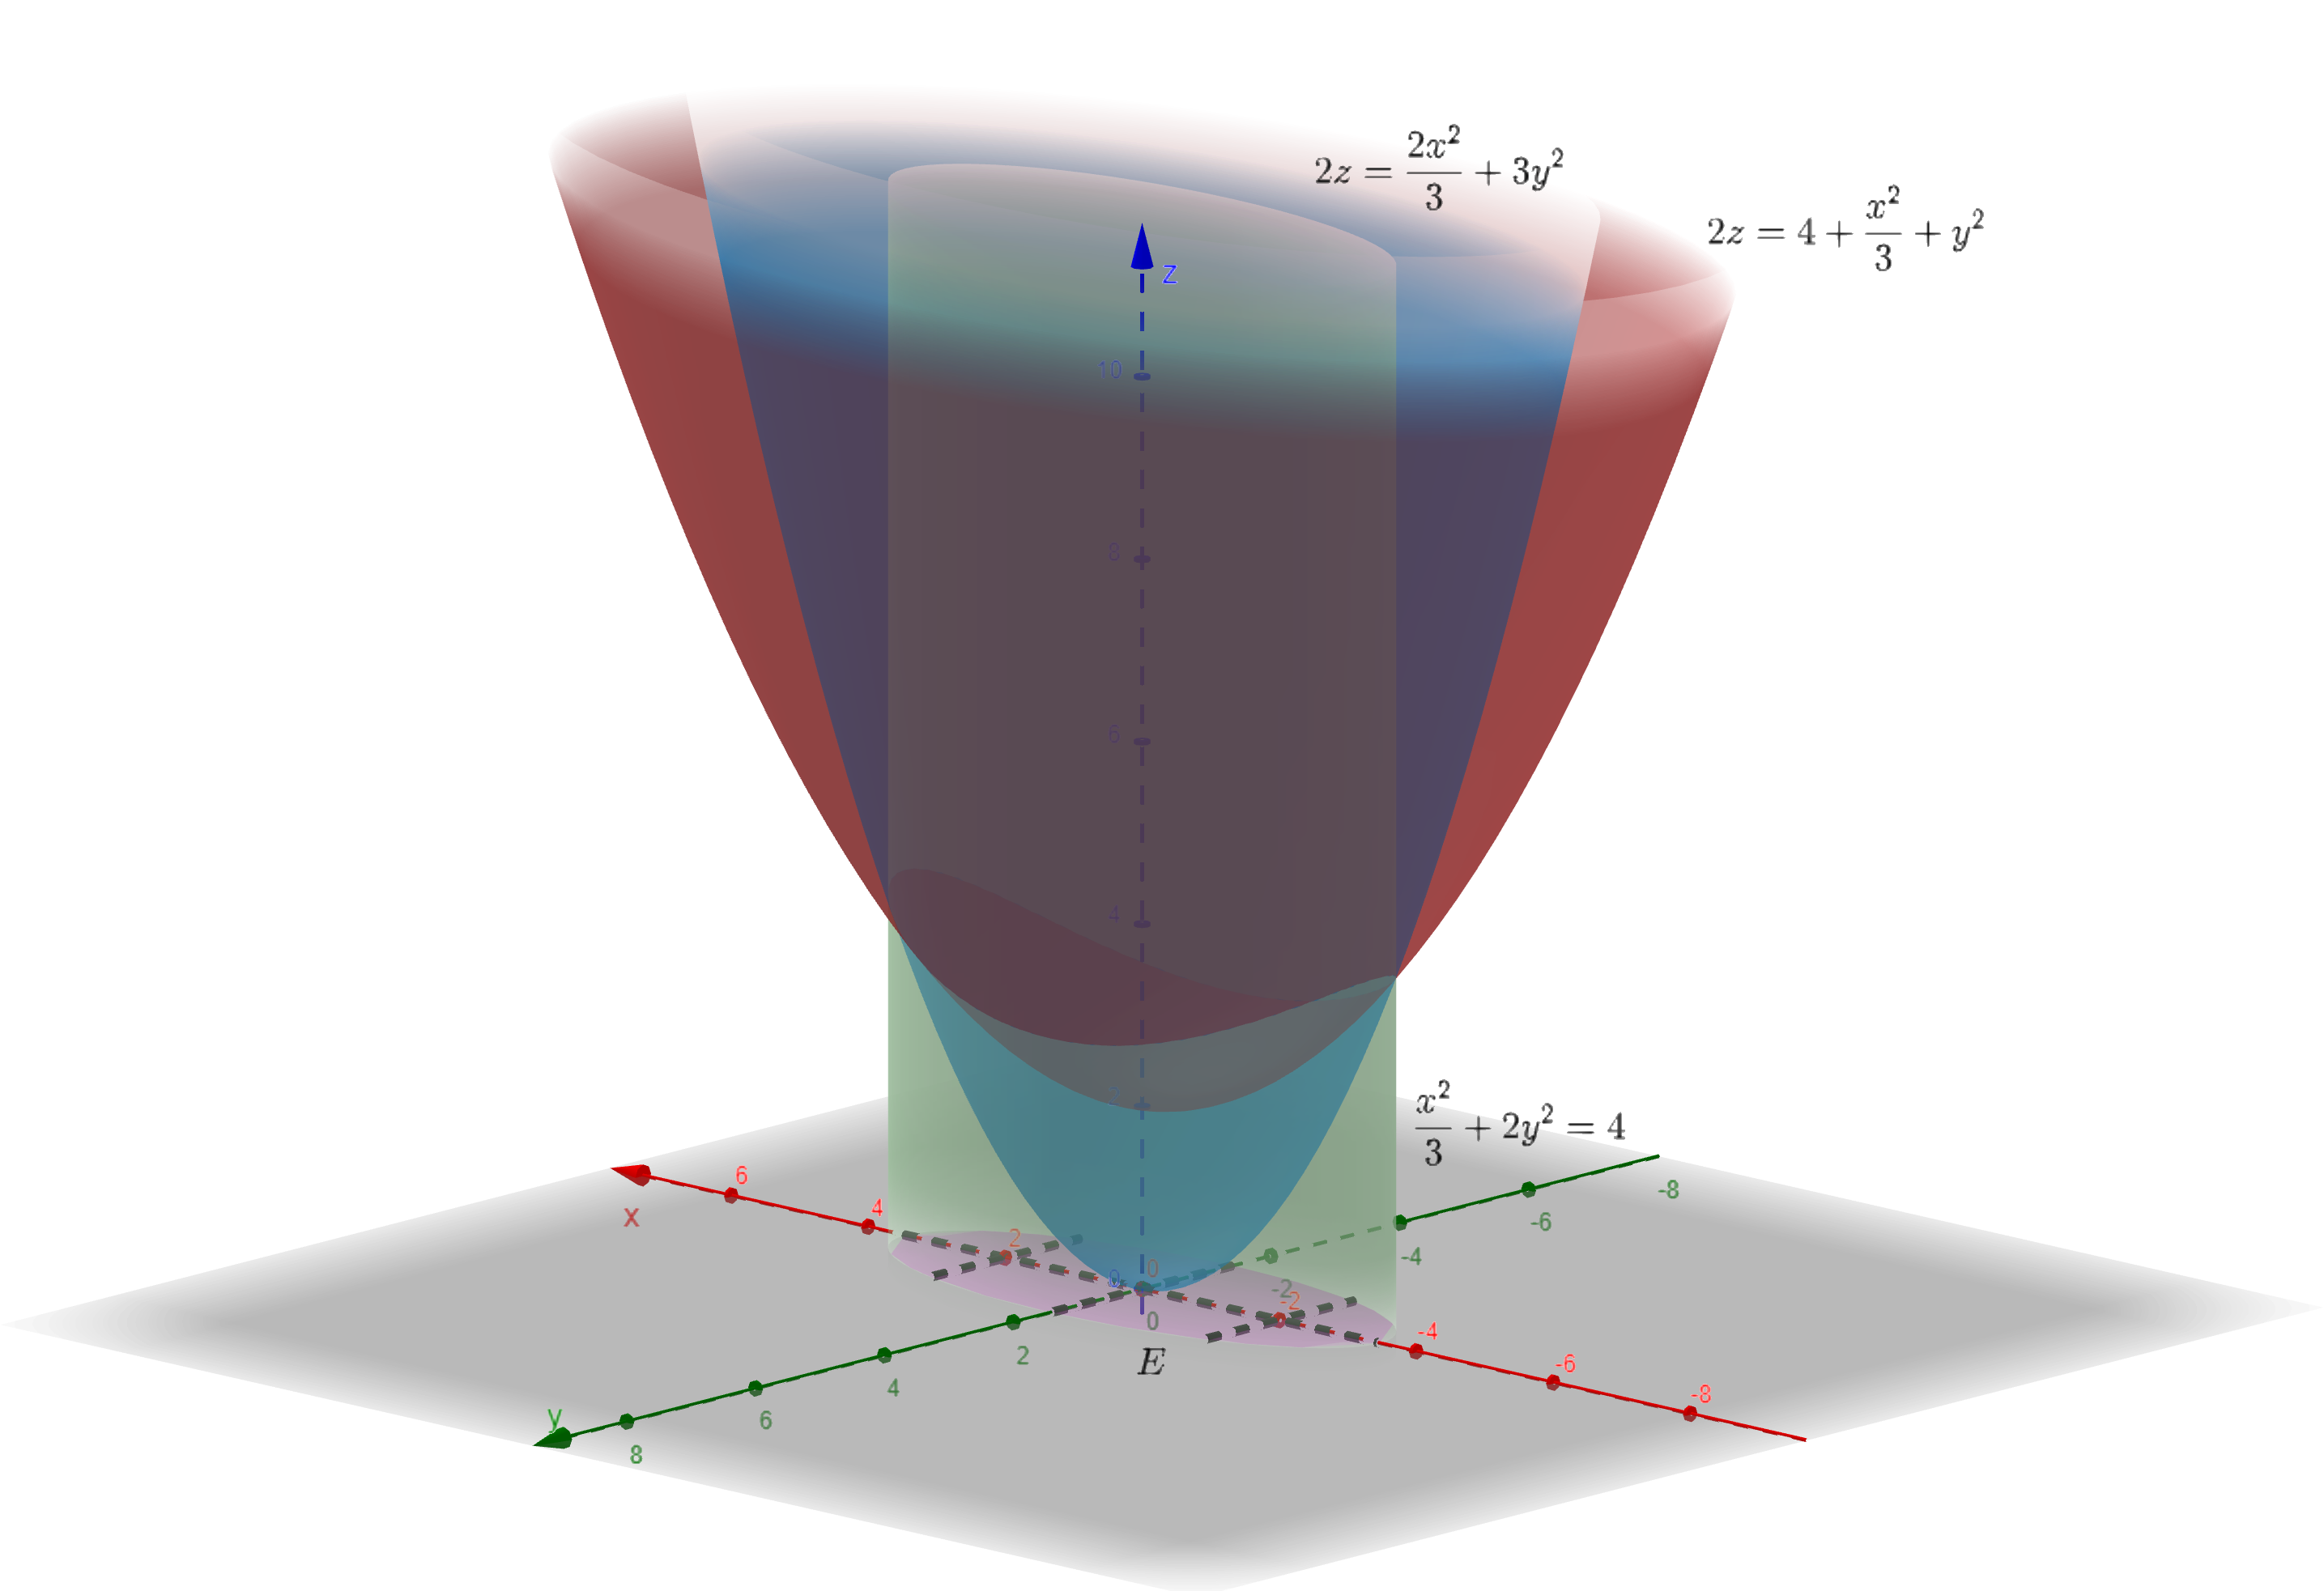
\includegraphics[width=0.6\textwidth]{images/Parabs.png}
    \end{center}

    \vspace{-2em}

    Haciendo el cambio de coordenadas elípticas: $$ a = \sqrt{12} = 2\sqrt{3},
        \quad b = \sqrt{2} $$ $$ x = 2\sqrt{3} r\cos\theta, \quad y = \sqrt{2}
        r\sin\theta $$ El jacobiano es: $$ J = 2\sqrt{6} $$ Finalmente, el cambio de
    variable nos ofrece que el volumen del conjunto es: $$ 2\sqrt{6} \pi. $$ }

\vspace{1em}

\begin{observación}
Sean $U, V \subset \mathbb{R}^n$ abiertos y $\varphi: U \to V$ difeomorfismo-$C^1$.
$$\varphi = \begin{cases} x_1 = x_1(u_1, \ldots, u_n) \\ \vdots \\ x_n = x_n(u_1, \ldots, u_n) \end{cases}$$
Entonces:
$$det(D_{\varphi}) = \frac{\partial{(x_1, \ldots, x_n)}}{\partial{(u_1, \ldots, u_n)}} = \begin{vmatrix} \frac{\partial{x_1}}{\partial{u_1}} & \cdots & \frac{\partial{x_1}}{\partial{u_n}} \\ \vdots & \ddots & \vdots \\ \frac{\partial{x_n}}{\partial{u_1}} & \cdots & \frac{\partial{x_n}}{\partial{u_n}} \end{vmatrix}$$
Entonces el Teorema de Cambio de Variable queda como:
$$\int_{D = \varphi(E)} f(x_1, \ldots, x_n)dx_1 \cdots dx_n = \int_{E = \varphi^{-1}(D)} f(x_1(u), \ldots, x_n(u))|\det(D_{\varphi})|du_1 \cdots du_n$$ $$
    = \int_{E = \varphi^{-1}(D)} f(x_1(u), \ldots, x_n(u))|\frac{\partial{(x_1, \ldots, x_n)}}{\partial{(u_1, \ldots, u_n)}}|du_1 \cdots du_n$$
\end{observación}

\ejemplo{
    Ejercicio 4 (Hoja 4)\\
    Calcula el área del recinto delimitado por las rectas $\begin{cases} x + y = a \\ x + y = b \\ 2x - 3y = c \\ 2x - 3y = d \end{cases}$
    Supongamos que $a < b, c < d$.\\
    \vspace{-1.5em}
    \begin{center}
    \begin{tikzpicture}[scale=0.7]
        % Ejes
        \draw[thick,->] (-2,0) -- (4,0) node[right] {\small $x$};
        \draw[thick,->] (0,-3) -- (0,4) node[above] {\small $y$};

        % Conjunto de rectas paralelas
        \draw[thick] (-2,0) -- (1,3) node[right] {\small $2x - 3y = d$};
        \draw[thick] (-1,-2) -- (3,2) node[right] {\small $2x - 3y = c$};

        \draw[thick] (-1,4) -- (4,-1) node[right] {\small $x + 4y = b$};
        \draw[thick] (-1,2) -- (3,-2) node[right] {\small $x + 4y = a$};

        % Región sombreada
        \fill[pattern=north east lines, pattern color=black, opacity=0.5]
        (0.5,2.5) -- (2,1) -- (1,0) -- (-0.5,1.5) -- cycle;
    \end{tikzpicture}
\end{center}
    Para ello tomemos el cambio de variable: $\varphi^{-1} = \psi = \begin{cases} u = x + y \\ v = 2x -3y \end{cases} $\\
    \[area(D) = \int_{D = \varphi(E)}1 dx dy = \int_{E}1 \left| \frac{\partial(x,y)}{\partial (u,v)} \right| du dv\]
    Donde
    \[\frac{\partial{(u, v)}}{\partial{(x, y)}} = \begin{vmatrix} \frac{\partial{x}}{\partial{u}} & \frac{\partial{x}}{\partial{v}} \\ \frac{\partial{y}}{\partial{u}} & \frac{\partial{y}}{\partial{v}} \end{vmatrix} = \begin{vmatrix} 1 & 1 \\ 2 & -3 \end{vmatrix} = -5 \implies \frac{\partial{(x,y)}}{\partial(u,v)} = \frac{1}{-5}\]
    Entonces la integral anterior queda de la forma: $$\int_{E}\frac{1}{5}dudv =
        \frac{1}{5}\cdot area(E) = \frac{1}{5}(b-a)(d-c)$$ }

\ejemplo{
    Ejercicio 6.b (Hoja 4)\\

    Sea el conjunto
    \[
        D = \{(x,y) \in \mathbb{R}^2 : 1 \leq x^2 - y^2 \leq 9, 2 \leq xy \leq 4\}
    \]
    queremos calcular la integral
    \[
        \int_{D} (x^2 + y^2) dx dy
    \]

    Para ello consideremos el cambio de variable ("hiperbólico"):
    \[
        \psi(x,y) = \begin{cases}
            u = x^2 - y^2 \\
            v = 2xy
        \end{cases}
    \]

    Si
    \[
        \begin{cases}
            x = r\cos(\theta) \\
            y = r\sin(\theta)
        \end{cases}
        \implies
        \begin{cases}
            u = r^2(\cos^2(\theta) - \sin^2(\theta)) = r^2\cos(2\theta) \\
            v = r^2 2\sin(\theta)\cos(\theta) = r^2\sin(2\theta)
        \end{cases}
    \]

    Sean
    \[
        V = \{(x,y) : x > 0, y > 0\}, \quad U = \{(u,v) : v > 0\}
    \]
    Entonces $\psi: V \to U$ es biyectiva y existe $\varphi = \psi^{-1}: U \to V$.
    Además el conjunto transformado es

    \[
        E = \psi(D) = \{(u,v) \in \mathbb{R}^2 : 1 \leq u \leq 9, 4 \leq v \leq 8\}
    \]

    \definecolor{ffttww}{rgb}{1,0.2,0.4}
\definecolor{wwwwww}{rgb}{0.4,0.4,0.4}
\definecolor{zzttff}{rgb}{0.6,0.2,1}
\definecolor{qqqqff}{rgb}{0,0,1}
\definecolor{qqwuqq}{rgb}{0,0.39215686274509803,0}

\begin{center}
    \begin{tikzpicture}[line cap=round,line join=round,>=triangle 45,x=1cm,y=1cm, scale=0.8]
        \begin{axis}[
                x=1cm,y=1cm,
                axis lines=middle,
                xmin=-6.980018499664145,
                xmax=8.311088929879618,
                ymin=-4.834155653613292,
                ymax=5.635191419227629,
                xtick={-6,-5,...,8},
                ytick={-4,-3,...,5},]
            \clip(-6.980018499664145,-4.834155653613292) rectangle (8.311088929879618,5.635191419227629);
            \draw[line width=2pt,color=qqwuqq,smooth,samples=100,domain=-6.980018499664145:-1.000000035933682] plot(\x,{sqrt((\x)^(2)-1)});
            \draw[line width=2pt,color=qqwuqq,smooth,samples=100,domain=1.0000017926861213:8.311088929879618] plot(\x,{sqrt((\x)^(2)-1)});
            \draw[line width=2pt,color=qqwuqq,smooth,samples=100,domain=-6.980018499664145:-1.000000035933682] plot(\x,{0-sqrt((\x)^(2)-1)});
            \draw[line width=2pt,color=qqwuqq,smooth,samples=100,domain=1.0000017926861213:8.311088929879618] plot(\x,{0-sqrt((\x)^(2)-1)});
            \draw[line width=2pt,color=qqqqff,smooth,samples=100,domain=-6.980018499664145:-3.000000126358707] plot(\x,{sqrt((\x)^(2)-9)});
            \draw[line width=2pt,color=qqqqff,smooth,samples=100,domain=3.000000036720542:8.311088929879618] plot(\x,{sqrt((\x)^(2)-9)});
            \draw[line width=2pt,color=qqqqff,smooth,samples=100,domain=-6.980018499664145:-3.000000126358707] plot(\x,{0-sqrt((\x)^(2)-9)});
            \draw[line width=2pt,color=qqqqff,smooth,samples=100,domain=3.000000036720542:8.311088929879618] plot(\x,{0-sqrt((\x)^(2)-9)});
            \draw[line width=2pt,color=zzttff,smooth,samples=100,domain=-6.980018499664145:8.311088929879618] plot(\x,{4/(\x)});
            \draw[line width=2pt,color=wwwwww,smooth,samples=100,domain=-6.980018499664145:8.311088929879618] plot(\x,{2/(\x)});
            \draw[line width=2pt,dash pattern=on 1pt off 1pt,color=qqqqff,fill=qqqqff,fill opacity=0.25](-6.3847153381513255,5.635191419227629)--(-6.048737592434519,5.2523543732435405)--(-5.6738198153857935,4.815831319457159)--(-5.34348710548939,4.4218609709636265)--(-5.051130148865137,4.063731755514177)--(-4.791434885181513,3.7360203772108056)--(-4.560084126973393,3.4342928304200706)--(-4.353538422272434,3.1548845928500064)--(-4.168872693913425,2.894736523080638)--(-4.003652814672324,2.651270612448609)--(-3.8558412250924663,2.4222946875065743)--(-3.723723976402839,2.2059284332084244)--(-3.605853789710893,2.0005453138513034)--(-3.5010052374186813,1.804726481335341)--(-3.4081392079271264,1.6172238127761225)--(-3.3263745603601285,1.4369299620409617)--(-3.254965410238351,1.2628538402555207)--(-3.1932828747352637,1.09410032358898)--(-3.1408003911094218,0.9298532662700562)--(-3.0970819340246734,0.7693611025142957)--(-3.061772617465393,0.6119244733305585)--(-3.0345912893929174,0.4568854272784041)--(-3.015324822566086,0.30361782817087024)--(-3.0038238806050486,0.1515186645043127)--(-3,0)--(-3.0038238806050486,-0.1515186645043127)--(-3.015324822566086,-0.30361782817087024)--(-3.0345912893929174,-0.4568854272784041)--(-3.061772617465393,-0.6119244733305585)--(-3.0970819340246734,-0.7693611025142957)--(-3.1408003911094218,-0.9298532662700562)--(-3.1932828747352637,-1.09410032358898)--(-3.254965410238351,-1.26285384025552)--(-3.3263745603601285,-1.4369299620409626)--(-3.4081392079271264,-1.6172238127761225)--(-3.5010052374186813,-1.804726481335341)--(-3.605853789710893,-2.000545313851303)--(-3.723723976402839,-2.2059284332084235)--(-3.8558412250924663,-2.422294687506574)--(-4.003652814672324,-2.6512706124486085)--(-4.168872693913425,-2.8947365230806383)--(-4.353538422272434,-3.154884592850007)--(-4.560084126973393,-3.4342928304200706)--(-4.791434885181513,-3.7360203772108065)--(-5.051130148865137,-4.063731755514177)--(-5.34348710548939,-4.4218609709636265)--(-5.6738198153857935,-4.815831319457158)--(-5.689558087552922,-4.834155653613292)--(-4.937225681200824,-4.834155653613292)--(-4.648495574090159,-4.539659800286337)--(-3.987074503787965,-3.8596325082520546)--(-3.482046043354327,-3.3353627460951714)--(-3.084627307869777,-2.9180345488797683)--(-2.7644603370004397,-2.5772545382341616)--(-2.50166742770917,-2.293107044789017)--(-2.282691237828824,-2.051993978368477)--(-2.0979708921863063,-1.844310674604744)--(-1.9405735159998447,-1.6630771392211485)--(-1.8053523464111376,-1.5030958368288427)--(-1.6884093121993098,-1.360413909632413)--(-1.5867409615357064,-1.2319687005014608)--(-1.4979987282400073,-1.1153475645773734)--(-1.4203227033128383,-1.0086211288416913)--(-1.3522239420743023,-0.9102250213650281)--(-1.2924995898018379,-0.8188743430086928)--(-1.2401706762957263,-0.7335007200704031)--(-1.1944358741971148,-0.6532052185714884)--(-1.1546367005053204,-0.5772225828515496)--(-1.1202310579323058,-0.5048936751001468)--(-1.0907729512342803,-0.43564392701418686)--(-1.0658968471637253,-0.3689662434336915)--(-1.0453055821243915,-0.3044072272801905)--(-1.0287610262529718,-0.2415558923666872)--(-1.0160769296743273,-0.18003423845593258)--(-1.0071135343575892,-0.11948920907862247)--(-1.001773652238346,-0.059585655311956046)--(-1,0)--(-1.001773652238346,0.059585655311956046)--(-1.0071135343575892,0.11948920907862247)--(-1.0160769296743273,0.18003423845593258)--(-1.0287610262529718,0.2415558923666872)--(-1.0453055821243915,0.3044072272801905)--(-1.0658968471637253,0.3689662434336915)--(-1.0907729512342803,0.43564392701418686)--(-1.1202310579323058,0.5048936751001468)--(-1.1546367005053204,0.5772225828515496)--(-1.1944358741971148,0.6532052185714884)--(-1.2401706762957263,0.7335007200704031)--(-1.2924995898018379,0.8188743430086928)--(-1.3522239420743023,0.9102250213650281)--(-1.4203227033128383,1.0086211288416913)--(-1.4979987282400073,1.1153475645773734)--(-1.5867409615357064,1.2319687005014608)--(-1.6884093121993098,1.3604139096324124)--(-1.8053523464111376,1.5030958368288427)--(-1.9405735159998447,1.6630771392211485)--(-2.0979708921863063,1.844310674604744)--(-2.282691237828824,2.051993978368477)--(-2.50166742770917,2.2931070447890165)--(-2.7644603370004397,2.577254538234162)--(-3.084627307869777,2.918034548879768)--(-3.482046043354327,3.3353627460951714)--(-3.987074503787965,3.8596325082520546)--(-4.648495574090159,4.539659800286338)--(-5.549981769018035,5.459148068740447)--(-5.723693021194804,5.635191419227629);
            \draw[line width=2pt,dash pattern=on 1pt off 1pt,color=qqqqff,fill=qqqqff,fill opacity=0.25](5.723693021194805,5.635191419227629)--(5.549981769018035,5.459148068740447)--(4.648495574090159,4.539659800286338)--(3.9870745037879645,3.8596325082520546)--(3.482046043354327,3.3353627460951714)--(3.084627307869777,2.918034548879768)--(2.7644603370004397,2.577254538234162)--(2.5016674277091706,2.2931070447890165)--(2.282691237828824,2.051993978368477)--(2.0979708921863063,1.844310674604744)--(1.9405735159998456,1.6630771392211485)--(1.8053523464111367,1.5030958368288427)--(1.688409312199309,1.3604139096324124)--(1.5867409615357064,1.2319687005014608)--(1.4979987282400073,1.1153475645773734)--(1.4203227033128383,1.0086211288416913)--(1.3522239420743032,0.9102250213650281)--(1.2924995898018379,0.8188743430086928)--(1.2401706762957272,0.7335007200704031)--(1.1944358741971148,0.6532052185714884)--(1.1546367005053204,0.5772225828515496)--(1.1202310579323058,0.5048936751001468)--(1.090772951234281,0.43564392701418686)--(1.0658968471637253,0.3689662434336915)--(1.0453055821243924,0.3044072272801905)--(1.0287610262529718,0.2415558923666872)--(1.0160769296743273,0.18003423845593258)--(1.0071135343575892,0.11948920907862247)--(1.001773652238347,0.059585655311956046)--(1,0)--(1.001773652238347,-0.059585655311956046)--(1.0071135343575892,-0.11948920907862247)--(1.0160769296743273,-0.18003423845593258)--(1.0287610262529718,-0.2415558923666872)--(1.0453055821243924,-0.3044072272801905)--(1.0658968471637253,-0.3689662434336915)--(1.090772951234281,-0.43564392701418686)--(1.1202310579323058,-0.5048936751001468)--(1.1546367005053204,-0.5772225828515496)--(1.1944358741971148,-0.6532052185714884)--(1.2401706762957272,-0.7335007200704031)--(1.2924995898018379,-0.8188743430086928)--(1.3522239420743032,-0.9102250213650281)--(1.4203227033128383,-1.0086211288416913)--(1.4979987282400073,-1.1153475645773734)--(1.5867409615357064,-1.2319687005014608)--(1.688409312199309,-1.360413909632413)--(1.8053523464111367,-1.5030958368288427)--(1.9405735159998456,-1.6630771392211485)--(2.0979708921863063,-1.844310674604744)--(2.282691237828824,-2.051993978368477)--(2.5016674277091706,-2.293107044789017)--(2.7644603370004397,-2.5772545382341616)--(3.084627307869777,-2.9180345488797683)--(3.482046043354327,-3.3353627460951714)--(3.9870745037879645,-3.8596325082520546)--(4.648495574090159,-4.539659800286337)--(4.937225681200824,-4.834155653613292)--(5.689558087552922,-4.834155653613292)--(5.673819815385794,-4.815831319457158)--(5.343487105489389,-4.4218609709636265)--(5.051130148865136,-4.063731755514177)--(4.791434885181513,-3.7360203772108065)--(4.5600841269733925,-3.4342928304200706)--(4.353538422272434,-3.154884592850007)--(4.168872693913424,-2.8947365230806383)--(4.003652814672324,-2.6512706124486085)--(3.8558412250924663,-2.422294687506574)--(3.72372397640284,-2.2059284332084235)--(3.6058537897108938,-2.000545313851303)--(3.5010052374186813,-1.804726481335341)--(3.4081392079271264,-1.6172238127761225)--(3.3263745603601285,-1.4369299620409626)--(3.254965410238351,-1.26285384025552)--(3.193282874735264,-1.09410032358898)--(3.1408003911094218,-0.9298532662700562)--(3.0970819340246734,-0.7693611025142957)--(3.061772617465393,-0.6119244733305585)--(3.0345912893929174,-0.4568854272784041)--(3.015324822566086,-0.30361782817087024)--(3.0038238806050486,-0.1515186645043127)--(3,0)--(3.0038238806050486,0.1515186645043127)--(3.015324822566086,0.30361782817087024)--(3.0345912893929174,0.4568854272784041)--(3.061772617465393,0.6119244733305585)--(3.0970819340246734,0.7693611025142957)--(3.1408003911094218,0.9298532662700562)--(3.193282874735264,1.09410032358898)--(3.254965410238351,1.2628538402555207)--(3.3263745603601285,1.4369299620409617)--(3.4081392079271264,1.6172238127761225)--(3.5010052374186813,1.804726481335341)--(3.6058537897108938,2.0005453138513034)--(3.72372397640284,2.2059284332084244)--(3.8558412250924663,2.4222946875065743)--(4.003652814672324,2.651270612448609)--(4.168872693913424,2.894736523080638)--(4.353538422272434,3.1548845928500064)--(4.5600841269733925,3.4342928304200706)--(4.791434885181513,3.7360203772108056)--(5.051130148865136,4.063731755514177)--(5.343487105489389,4.4218609709636265)--(5.673819815385794,4.815831319457159)--(6.048737592434518,5.2523543732435405)--(6.3847153381513255,5.635191419227629);
            \draw[line width=2pt,dash pattern=on 1pt off 1pt,color=qqqqff,fill=qqqqff,fill opacity=0.25](-6.3847153381513255,5.635191419227629)--(-6.048737592434519,5.2523543732435405)--(-5.6738198153857935,4.815831319457159)--(-5.34348710548939,4.4218609709636265)--(-5.051130148865137,4.063731755514177)--(-4.791434885181513,3.7360203772108056)--(-4.560084126973393,3.4342928304200706)--(-4.353538422272434,3.1548845928500064)--(-4.168872693913425,2.894736523080638)--(-4.003652814672324,2.651270612448609)--(-3.8558412250924663,2.4222946875065743)--(-3.723723976402839,2.2059284332084244)--(-3.605853789710893,2.0005453138513034)--(-3.5010052374186813,1.804726481335341)--(-3.4081392079271264,1.6172238127761225)--(-3.3263745603601285,1.4369299620409617)--(-3.254965410238351,1.2628538402555207)--(-3.1932828747352637,1.09410032358898)--(-3.1408003911094218,0.9298532662700562)--(-3.0970819340246734,0.7693611025142957)--(-3.061772617465393,0.6119244733305585)--(-3.0345912893929174,0.4568854272784041)--(-3.015324822566086,0.30361782817087024)--(-3.0038238806050486,0.1515186645043127)--(-3,0)--(-3.0038238806050486,-0.1515186645043127)--(-3.015324822566086,-0.30361782817087024)--(-3.0345912893929174,-0.4568854272784041)--(-3.061772617465393,-0.6119244733305585)--(-3.0970819340246734,-0.7693611025142957)--(-3.1408003911094218,-0.9298532662700562)--(-3.1932828747352637,-1.09410032358898)--(-3.254965410238351,-1.26285384025552)--(-3.3263745603601285,-1.4369299620409626)--(-3.4081392079271264,-1.6172238127761225)--(-3.5010052374186813,-1.804726481335341)--(-3.605853789710893,-2.000545313851303)--(-3.723723976402839,-2.2059284332084235)--(-3.8558412250924663,-2.422294687506574)--(-4.003652814672324,-2.6512706124486085)--(-4.168872693913425,-2.8947365230806383)--(-4.353538422272434,-3.154884592850007)--(-4.560084126973393,-3.4342928304200706)--(-4.791434885181513,-3.7360203772108065)--(-5.051130148865137,-4.063731755514177)--(-5.34348710548939,-4.4218609709636265)--(-5.6738198153857935,-4.815831319457158)--(-5.689558087552922,-4.834155653613292)--(-4.937225681200824,-4.834155653613292)--(-4.648495574090159,-4.539659800286337)--(-3.987074503787965,-3.8596325082520546)--(-3.482046043354327,-3.3353627460951714)--(-3.084627307869777,-2.9180345488797683)--(-2.7644603370004397,-2.5772545382341616)--(-2.50166742770917,-2.293107044789017)--(-2.282691237828824,-2.051993978368477)--(-2.0979708921863063,-1.844310674604744)--(-1.9405735159998447,-1.6630771392211485)--(-1.8053523464111376,-1.5030958368288427)--(-1.6884093121993098,-1.360413909632413)--(-1.5867409615357064,-1.2319687005014608)--(-1.4979987282400073,-1.1153475645773734)--(-1.4203227033128383,-1.0086211288416913)--(-1.3522239420743023,-0.9102250213650281)--(-1.2924995898018379,-0.8188743430086928)--(-1.2401706762957263,-0.7335007200704031)--(-1.1944358741971148,-0.6532052185714884)--(-1.1546367005053204,-0.5772225828515496)--(-1.1202310579323058,-0.5048936751001468)--(-1.0907729512342803,-0.43564392701418686)--(-1.0658968471637253,-0.3689662434336915)--(-1.0453055821243915,-0.3044072272801905)--(-1.0287610262529718,-0.2415558923666872)--(-1.0160769296743273,-0.18003423845593258)--(-1.0071135343575892,-0.11948920907862247)--(-1.001773652238346,-0.059585655311956046)--(-1,0)--(-1.001773652238346,0.059585655311956046)--(-1.0071135343575892,0.11948920907862247)--(-1.0160769296743273,0.18003423845593258)--(-1.0287610262529718,0.2415558923666872)--(-1.0453055821243915,0.3044072272801905)--(-1.0658968471637253,0.3689662434336915)--(-1.0907729512342803,0.43564392701418686)--(-1.1202310579323058,0.5048936751001468)--(-1.1546367005053204,0.5772225828515496)--(-1.1944358741971148,0.6532052185714884)--(-1.2401706762957263,0.7335007200704031)--(-1.2924995898018379,0.8188743430086928)--(-1.3522239420743023,0.9102250213650281)--(-1.4203227033128383,1.0086211288416913)--(-1.4979987282400073,1.1153475645773734)--(-1.5867409615357064,1.2319687005014608)--(-1.6884093121993098,1.3604139096324124)--(-1.8053523464111376,1.5030958368288427)--(-1.9405735159998447,1.6630771392211485)--(-2.0979708921863063,1.844310674604744)--(-2.282691237828824,2.051993978368477)--(-2.50166742770917,2.2931070447890165)--(-2.7644603370004397,2.577254538234162)--(-3.084627307869777,2.918034548879768)--(-3.482046043354327,3.3353627460951714)--(-3.987074503787965,3.8596325082520546)--(-4.648495574090159,4.539659800286338)--(-5.549981769018035,5.459148068740447)--(-5.723693021194804,5.635191419227629);
            \draw[line width=2pt,dash pattern=on 1pt off 1pt,color=qqqqff,fill=qqqqff,fill opacity=0.25](5.723693021194805,5.635191419227629)--(5.549981769018035,5.459148068740447)--(4.648495574090159,4.539659800286338)--(3.9870745037879645,3.8596325082520546)--(3.482046043354327,3.3353627460951714)--(3.084627307869777,2.918034548879768)--(2.7644603370004397,2.577254538234162)--(2.5016674277091706,2.2931070447890165)--(2.282691237828824,2.051993978368477)--(2.0979708921863063,1.844310674604744)--(1.9405735159998456,1.6630771392211485)--(1.8053523464111367,1.5030958368288427)--(1.688409312199309,1.3604139096324124)--(1.5867409615357064,1.2319687005014608)--(1.4979987282400073,1.1153475645773734)--(1.4203227033128383,1.0086211288416913)--(1.3522239420743032,0.9102250213650281)--(1.2924995898018379,0.8188743430086928)--(1.2401706762957272,0.7335007200704031)--(1.1944358741971148,0.6532052185714884)--(1.1546367005053204,0.5772225828515496)--(1.1202310579323058,0.5048936751001468)--(1.090772951234281,0.43564392701418686)--(1.0658968471637253,0.3689662434336915)--(1.0453055821243924,0.3044072272801905)--(1.0287610262529718,0.2415558923666872)--(1.0160769296743273,0.18003423845593258)--(1.0071135343575892,0.11948920907862247)--(1.001773652238347,0.059585655311956046)--(1,0)--(1.001773652238347,-0.059585655311956046)--(1.0071135343575892,-0.11948920907862247)--(1.0160769296743273,-0.18003423845593258)--(1.0287610262529718,-0.2415558923666872)--(1.0453055821243924,-0.3044072272801905)--(1.0658968471637253,-0.3689662434336915)--(1.090772951234281,-0.43564392701418686)--(1.1202310579323058,-0.5048936751001468)--(1.1546367005053204,-0.5772225828515496)--(1.1944358741971148,-0.6532052185714884)--(1.2401706762957272,-0.7335007200704031)--(1.2924995898018379,-0.8188743430086928)--(1.3522239420743032,-0.9102250213650281)--(1.4203227033128383,-1.0086211288416913)--(1.4979987282400073,-1.1153475645773734)--(1.5867409615357064,-1.2319687005014608)--(1.688409312199309,-1.360413909632413)--(1.8053523464111367,-1.5030958368288427)--(1.9405735159998456,-1.6630771392211485)--(2.0979708921863063,-1.844310674604744)--(2.282691237828824,-2.051993978368477)--(2.5016674277091706,-2.293107044789017)--(2.7644603370004397,-2.5772545382341616)--(3.084627307869777,-2.9180345488797683)--(3.482046043354327,-3.3353627460951714)--(3.9870745037879645,-3.8596325082520546)--(4.648495574090159,-4.539659800286337)--(4.937225681200824,-4.834155653613292)--(5.689558087552922,-4.834155653613292)--(5.673819815385794,-4.815831319457158)--(5.343487105489389,-4.4218609709636265)--(5.051130148865136,-4.063731755514177)--(4.791434885181513,-3.7360203772108065)--(4.5600841269733925,-3.4342928304200706)--(4.353538422272434,-3.154884592850007)--(4.168872693913424,-2.8947365230806383)--(4.003652814672324,-2.6512706124486085)--(3.8558412250924663,-2.422294687506574)--(3.72372397640284,-2.2059284332084235)--(3.6058537897108938,-2.000545313851303)--(3.5010052374186813,-1.804726481335341)--(3.4081392079271264,-1.6172238127761225)--(3.3263745603601285,-1.4369299620409626)--(3.254965410238351,-1.26285384025552)--(3.193282874735264,-1.09410032358898)--(3.1408003911094218,-0.9298532662700562)--(3.0970819340246734,-0.7693611025142957)--(3.061772617465393,-0.6119244733305585)--(3.0345912893929174,-0.4568854272784041)--(3.015324822566086,-0.30361782817087024)--(3.0038238806050486,-0.1515186645043127)--(3,0)--(3.0038238806050486,0.1515186645043127)--(3.015324822566086,0.30361782817087024)--(3.0345912893929174,0.4568854272784041)--(3.061772617465393,0.6119244733305585)--(3.0970819340246734,0.7693611025142957)--(3.1408003911094218,0.9298532662700562)--(3.193282874735264,1.09410032358898)--(3.254965410238351,1.2628538402555207)--(3.3263745603601285,1.4369299620409617)--(3.4081392079271264,1.6172238127761225)--(3.5010052374186813,1.804726481335341)--(3.6058537897108938,2.0005453138513034)--(3.72372397640284,2.2059284332084244)--(3.8558412250924663,2.4222946875065743)--(4.003652814672324,2.651270612448609)--(4.168872693913424,2.894736523080638)--(4.353538422272434,3.1548845928500064)--(4.5600841269733925,3.4342928304200706)--(4.791434885181513,3.7360203772108056)--(5.051130148865136,4.063731755514177)--(5.343487105489389,4.4218609709636265)--(5.673819815385794,4.815831319457159)--(6.048737592434518,5.2523543732435405)--(6.3847153381513255,5.635191419227629);
            \draw[line width=2pt,dash pattern=on 1pt off 1pt,color=ffttww,fill=ffttww,fill opacity=0.25](0.35529615458839425,5.635191419227629)--(0.3802397600827543,5.259839211882339)--(0.41203075536781275,4.854006585539074)--(0.44496850163930257,4.4947001700835605)--(0.4791161861853807,4.17435281392509)--(0.5145417254096805,3.8869539655070575)--(0.5513182156927343,3.6276689996302554)--(0.5895244368367559,3.3925650490953574)--(0.6292454153904545,3.1784101259744135)--(0.6705730563311612,2.9825236506554536)--(0.7136068529813463,2.8026636678785932)--(0.7584546867021562,2.636940657188393)--(0.8052337298946451,2.4837508983406287)--(0.8540714682213387,2.341724404124088)--(0.9051068608249484,2.2096838357595967)--(0.9584916607786166,2.0866117900027734)--(1.0143919221927589,1.9716245331259183)--(1.0729897255042782,1.8639507466486245)--(1.1344851587096532,1.7629142035447791)--(1.1990985999619026,1.667919552289982)--(1.2670733564027699,1.578440577172276)--(1.3386787258244504,1.4940104458358834)--(1.4142135623730943,1.414213562373095)--(1.4940104458358836,1.3386787258244504)--(1.5784405771722758,1.2670733564027694)--(1.667919552289981,1.199098599961902)--(1.7629142035447798,1.134485158709653)--(1.8639507466486238,1.0729897255042777)--(1.9716245331259186,1.014391922192758)--(2.0866117900027734,0.9584916607786165)--(2.2096838357595976,0.9051068608249484)--(2.341724404124088,0.8540714682213387)--(2.4837508983406282,0.8052337298946445)--(2.6369406571883927,0.7584546867021557)--(2.802663667878593,0.7136068529813457)--(2.982523650655452,0.6705730563311615)--(3.178410125974413,0.629245415390455)--(3.3925650490953574,0.5895244368367557)--(3.627668999630256,0.5513182156927341)--(3.8869539655070575,0.5145417254096804)--(4.17435281392509,0.47911618618538065)--(4.4947001700835605,0.44496850163930257)--(4.854006585539075,0.4120307553678128)--(5.259839211882338,0.3802397600827544)--(5.721860590674567,0.34953665303547954)--(6.252607879196409,0.319866532275976)--(6.868647747495386,0.29117812901808604)--(7.592336708420492,0.26342351199754355)--(8.311088929879634,0.2410290285429407)--(8.31108892987962,0.2410290285429407)--(8.31108892987962,0.4815730493748811)--(7.731504521126992,0.5173637277284985)--(7.1607964118688345,0.558597084727908)--(6.653318942019616,0.6012037052271244)--(6.199115383430095,0.6452533551306026)--(5.790215225984317,0.6908206075051402)--(5.420162428412655,0.7379852638791555)--(5.083672026731743,0.786832820639606)--(4.776376122446434,0.8374549862608431)--(4.494633237379147,0.8899502559484541)--(4.235383329038813,0.9444245512737965)--(3.996036197671181,1.000991933539324)--(3.774384644411156,1.0597754009843487)--(3.568536204150886,1.1209077815568302)--(3.3768589775398623,1.184532734889069)--(3.197938277971775,1.2508058793858001)--(3.0305416555249725,1.319896063037975)--(2.8735904683498488,1.3919867998090174)--(2.7261366148203394,1.4672778973197609)--(2.587343365550368,1.5459873062302794)--(2.456469476510074,1.6283532273654928)--(2.3328559461638867,1.714636519489144)--(2.215914917107206,1.8051234589917597)--(2.1051203276984425,1.9001289129981742)--(2,2)--(1.9001289129981744,2.1051203276984416)--(1.8051234589917606,2.215914917107206)--(1.714636519489143,2.3328559461638863)--(1.6283532273654926,2.456469476510073)--(1.5459873062302796,2.587343365550369)--(1.4672778973197604,2.7261366148203385)--(1.3919867998090174,2.8735904683498488)--(1.319896063037975,3.0305416555249725)--(1.2508058793858,3.197938277971774)--(1.1845327348890695,3.3768589775398636)--(1.1209077815568298,3.568536204150886)--(1.059775400984349,3.774384644411156)--(1.0009919335393243,3.9960361976711805)--(0.9444245512737967,4.235383329038812)--(0.8899502559484541,4.494633237379147)--(0.8374549862608438,4.776376122446434)--(0.7868328206396066,5.083672026731743)--(0.737985263879156,5.420162428412655)--(0.7105789896156135,5.635191419227629);
            \draw[line width=2pt,dash pattern=on 1pt off 1pt,color=ffttww,fill=ffttww,fill opacity=0.25](-6.980018499664146,-0.2869068844079955)--(-6.980018499664146,-0.5737747750837652)--(-6.980018499664159,-0.5737747750837652)--(-6.653318942019615,-0.6012037052271244)--(-6.199115383430094,-0.6452533551306026)--(-5.790215225984318,-0.6908206075051402)--(-5.420162428412655,-0.7379852638791555)--(-5.083672026731743,-0.786832820639606)--(-4.776376122446434,-0.8374549862608431)--(-4.494633237379147,-0.8899502559484541)--(-4.235383329038812,-0.9444245512737965)--(-3.9960361976711805,-1.000991933539324)--(-3.7743846444111555,-1.0597754009843487)--(-3.568536204150886,-1.1209077815568302)--(-3.376858977539863,-1.184532734889069)--(-3.197938277971774,-1.2508058793858001)--(-3.0305416555249725,-1.319896063037975)--(-2.8735904683498488,-1.3919867998090174)--(-2.7261366148203385,-1.4672778973197618)--(-2.587343365550369,-1.5459873062302794)--(-2.456469476510073,-1.6283532273654922)--(-2.332855946163886,-1.714636519489144)--(-2.215914917107206,-1.8051234589917597)--(-2.1051203276984425,-1.9001289129981733)--(-2,-2)--(-1.9001289129981744,-2.105120327698441)--(-1.8051234589917606,-2.215914917107206)--(-1.714636519489144,-2.3328559461638867)--(-1.6283532273654926,-2.4564694765100734)--(-1.5459873062302796,-2.587343365550369)--(-1.467277897319761,-2.7261366148203385)--(-1.3919867998090167,-2.8735904683498488)--(-1.319896063037975,-3.0305416555249725)--(-1.2508058793858008,-3.1979382779717747)--(-1.1845327348890689,-3.3768589775398636)--(-1.1209077815568298,-3.568536204150885)--(-1.059775400984349,-3.7743846444111564)--(-1.0009919335393236,-3.996036197671181)--(-0.9444245512737967,-4.235383329038812)--(-0.8899502559484541,-4.494633237379148)--(-0.837454986260843,-4.776376122446434)--(-0.8279367175320462,-4.834155653613292)--(-0.4138504973231439,-4.834155653613292)--(-0.44496850163930257,-4.4947001700835605)--(-0.47911618618537993,-4.174352813925089)--(-0.5145417254096805,-3.8869539655070575)--(-0.5513182156927343,-3.6276689996302562)--(-0.5895244368367552,-3.392565049095357)--(-0.6292454153904553,-3.1784101259744144)--(-0.6705730563311612,-2.982523650655454)--(-0.7136068529813463,-2.8026636678785932)--(-0.7584546867021562,-2.6369406571883935)--(-0.8052337298946451,-2.483750898340629)--(-0.8540714682213387,-2.341724404124088)--(-0.9051068608249484,-2.2096838357595976)--(-0.9584916607786166,-2.0866117900027734)--(-1.0143919221927582,-1.971624533125919)--(-1.0729897255042773,-1.8639507466486245)--(-1.1344851587096525,-1.7629142035447791)--(-1.1990985999619017,-1.667919552289982)--(-1.2670733564027692,-1.5784405771722754)--(-1.3386787258244504,-1.4940104458358834)--(-1.4142135623730951,-1.4142135623730943)--(-1.4940104458358836,-1.3386787258244504)--(-1.5784405771722758,-1.2670733564027685)--(-1.6679195522899817,-1.1990985999619013)--(-1.7629142035447798,-1.134485158709653)--(-1.8639507466486238,-1.0729897255042777)--(-1.9716245331259186,-1.014391922192758)--(-2.0866117900027734,-0.9584916607786165)--(-2.2096838357595967,-0.9051068608249484)--(-2.341724404124088,-0.8540714682213387)--(-2.483750898340629,-0.8052337298946445)--(-2.6369406571883927,-0.7584546867021557)--(-2.802663667878593,-0.7136068529813457)--(-2.982523650655453,-0.6705730563311615)--(-3.178410125974413,-0.629245415390455)--(-3.3925650490953574,-0.5895244368367557)--(-3.627668999630256,-0.5513182156927341)--(-3.8869539655070575,-0.5145417254096804)--(-4.17435281392509,-0.47911618618538065)--(-4.4947001700835605,-0.44496850163930257)--(-4.854006585539075,-0.4120307553678128)--(-5.259839211882338,-0.3802397600827544)--(-5.721860590674567,-0.34953665303547954)--(-6.25260787919641,-0.319866532275976)--(-6.868647747495386,-0.29117812901808604)--(-6.980018499664135,-0.2869068844079955);
            \draw[line width=2pt,dash pattern=on 1pt off 1pt,color=ffttww,fill=ffttww,fill opacity=0.25](0.35529615458839425,5.635191419227629)--(0.3802397600827543,5.259839211882339)--(0.41203075536781275,4.854006585539074)--(0.44496850163930257,4.4947001700835605)--(0.4791161861853807,4.17435281392509)--(0.5145417254096805,3.8869539655070575)--(0.5513182156927343,3.6276689996302554)--(0.5895244368367559,3.3925650490953574)--(0.6292454153904545,3.1784101259744135)--(0.6705730563311612,2.9825236506554536)--(0.7136068529813463,2.8026636678785932)--(0.7584546867021562,2.636940657188393)--(0.8052337298946451,2.4837508983406287)--(0.8540714682213387,2.341724404124088)--(0.9051068608249484,2.2096838357595967)--(0.9584916607786166,2.0866117900027734)--(1.0143919221927589,1.9716245331259183)--(1.0729897255042782,1.8639507466486245)--(1.1344851587096532,1.7629142035447791)--(1.1990985999619026,1.667919552289982)--(1.2670733564027699,1.578440577172276)--(1.3386787258244504,1.4940104458358834)--(1.4142135623730943,1.414213562373095)--(1.4940104458358836,1.3386787258244504)--(1.5784405771722758,1.2670733564027694)--(1.667919552289981,1.199098599961902)--(1.7629142035447798,1.134485158709653)--(1.8639507466486238,1.0729897255042777)--(1.9716245331259186,1.014391922192758)--(2.0866117900027734,0.9584916607786165)--(2.2096838357595976,0.9051068608249484)--(2.341724404124088,0.8540714682213387)--(2.4837508983406282,0.8052337298946445)--(2.6369406571883927,0.7584546867021557)--(2.802663667878593,0.7136068529813457)--(2.982523650655452,0.6705730563311615)--(3.178410125974413,0.629245415390455)--(3.3925650490953574,0.5895244368367557)--(3.627668999630256,0.5513182156927341)--(3.8869539655070575,0.5145417254096804)--(4.17435281392509,0.47911618618538065)--(4.4947001700835605,0.44496850163930257)--(4.854006585539075,0.4120307553678128)--(5.259839211882338,0.3802397600827544)--(5.721860590674567,0.34953665303547954)--(6.252607879196409,0.319866532275976)--(6.868647747495386,0.29117812901808604)--(7.592336708420492,0.26342351199754355)--(8.311088929879634,0.2410290285429407)--(8.31108892987962,0.2410290285429407)--(8.31108892987962,0.4815730493748811)--(7.731504521126992,0.5173637277284985)--(7.1607964118688345,0.558597084727908)--(6.653318942019616,0.6012037052271244)--(6.199115383430095,0.6452533551306026)--(5.790215225984317,0.6908206075051402)--(5.420162428412655,0.7379852638791555)--(5.083672026731743,0.786832820639606)--(4.776376122446434,0.8374549862608431)--(4.494633237379147,0.8899502559484541)--(4.235383329038813,0.9444245512737965)--(3.996036197671181,1.000991933539324)--(3.774384644411156,1.0597754009843487)--(3.568536204150886,1.1209077815568302)--(3.3768589775398623,1.184532734889069)--(3.197938277971775,1.2508058793858001)--(3.0305416555249725,1.319896063037975)--(2.8735904683498488,1.3919867998090174)--(2.7261366148203394,1.4672778973197609)--(2.587343365550368,1.5459873062302794)--(2.456469476510074,1.6283532273654928)--(2.3328559461638867,1.714636519489144)--(2.215914917107206,1.8051234589917597)--(2.1051203276984425,1.9001289129981742)--(2,2)--(1.9001289129981744,2.1051203276984416)--(1.8051234589917606,2.215914917107206)--(1.714636519489143,2.3328559461638863)--(1.6283532273654926,2.456469476510073)--(1.5459873062302796,2.587343365550369)--(1.4672778973197604,2.7261366148203385)--(1.3919867998090174,2.8735904683498488)--(1.319896063037975,3.0305416555249725)--(1.2508058793858,3.197938277971774)--(1.1845327348890695,3.3768589775398636)--(1.1209077815568298,3.568536204150886)--(1.059775400984349,3.774384644411156)--(1.0009919335393243,3.9960361976711805)--(0.9444245512737967,4.235383329038812)--(0.8899502559484541,4.494633237379147)--(0.8374549862608438,4.776376122446434)--(0.7868328206396066,5.083672026731743)--(0.737985263879156,5.420162428412655)--(0.7105789896156135,5.635191419227629);
            \draw[line width=2pt,dash pattern=on 1pt off 1pt,color=ffttww,fill=ffttww,fill opacity=0.25](-6.980018499664146,-0.2869068844079955)--(-6.980018499664146,-0.5737747750837652)--(-6.980018499664159,-0.5737747750837652)--(-6.653318942019615,-0.6012037052271244)--(-6.199115383430094,-0.6452533551306026)--(-5.790215225984318,-0.6908206075051402)--(-5.420162428412655,-0.7379852638791555)--(-5.083672026731743,-0.786832820639606)--(-4.776376122446434,-0.8374549862608431)--(-4.494633237379147,-0.8899502559484541)--(-4.235383329038812,-0.9444245512737965)--(-3.9960361976711805,-1.000991933539324)--(-3.7743846444111555,-1.0597754009843487)--(-3.568536204150886,-1.1209077815568302)--(-3.376858977539863,-1.184532734889069)--(-3.197938277971774,-1.2508058793858001)--(-3.0305416555249725,-1.319896063037975)--(-2.8735904683498488,-1.3919867998090174)--(-2.7261366148203385,-1.4672778973197618)--(-2.587343365550369,-1.5459873062302794)--(-2.456469476510073,-1.6283532273654922)--(-2.332855946163886,-1.714636519489144)--(-2.215914917107206,-1.8051234589917597)--(-2.1051203276984425,-1.9001289129981733)--(-2,-2)--(-1.9001289129981744,-2.105120327698441)--(-1.8051234589917606,-2.215914917107206)--(-1.714636519489144,-2.3328559461638867)--(-1.6283532273654926,-2.4564694765100734)--(-1.5459873062302796,-2.587343365550369)--(-1.467277897319761,-2.7261366148203385)--(-1.3919867998090167,-2.8735904683498488)--(-1.319896063037975,-3.0305416555249725)--(-1.2508058793858008,-3.1979382779717747)--(-1.1845327348890689,-3.3768589775398636)--(-1.1209077815568298,-3.568536204150885)--(-1.059775400984349,-3.7743846444111564)--(-1.0009919335393236,-3.996036197671181)--(-0.9444245512737967,-4.235383329038812)--(-0.8899502559484541,-4.494633237379148)--(-0.837454986260843,-4.776376122446434)--(-0.8279367175320462,-4.834155653613292)--(-0.4138504973231439,-4.834155653613292)--(-0.44496850163930257,-4.4947001700835605)--(-0.47911618618537993,-4.174352813925089)--(-0.5145417254096805,-3.8869539655070575)--(-0.5513182156927343,-3.6276689996302562)--(-0.5895244368367552,-3.392565049095357)--(-0.6292454153904553,-3.1784101259744144)--(-0.6705730563311612,-2.982523650655454)--(-0.7136068529813463,-2.8026636678785932)--(-0.7584546867021562,-2.6369406571883935)--(-0.8052337298946451,-2.483750898340629)--(-0.8540714682213387,-2.341724404124088)--(-0.9051068608249484,-2.2096838357595976)--(-0.9584916607786166,-2.0866117900027734)--(-1.0143919221927582,-1.971624533125919)--(-1.0729897255042773,-1.8639507466486245)--(-1.1344851587096525,-1.7629142035447791)--(-1.1990985999619017,-1.667919552289982)--(-1.2670733564027692,-1.5784405771722754)--(-1.3386787258244504,-1.4940104458358834)--(-1.4142135623730951,-1.4142135623730943)--(-1.4940104458358836,-1.3386787258244504)--(-1.5784405771722758,-1.2670733564027685)--(-1.6679195522899817,-1.1990985999619013)--(-1.7629142035447798,-1.134485158709653)--(-1.8639507466486238,-1.0729897255042777)--(-1.9716245331259186,-1.014391922192758)--(-2.0866117900027734,-0.9584916607786165)--(-2.2096838357595967,-0.9051068608249484)--(-2.341724404124088,-0.8540714682213387)--(-2.483750898340629,-0.8052337298946445)--(-2.6369406571883927,-0.7584546867021557)--(-2.802663667878593,-0.7136068529813457)--(-2.982523650655453,-0.6705730563311615)--(-3.178410125974413,-0.629245415390455)--(-3.3925650490953574,-0.5895244368367557)--(-3.627668999630256,-0.5513182156927341)--(-3.8869539655070575,-0.5145417254096804)--(-4.17435281392509,-0.47911618618538065)--(-4.4947001700835605,-0.44496850163930257)--(-4.854006585539075,-0.4120307553678128)--(-5.259839211882338,-0.3802397600827544)--(-5.721860590674567,-0.34953665303547954)--(-6.25260787919641,-0.319866532275976)--(-6.868647747495386,-0.29117812901808604)--(-6.980018499664135,-0.2869068844079955);
            \node[below] at (2.5,1.5) {\small $D^+$};
            \node[below] at (-2.5,-0.9) {\small $D^-$};
            
             % Add legend
        \node[draw,fill=qqqqff, fill opacity=0.6, minimum size=0.5cm,label=right:{$1 \leq x^2 + y^2 \leq 9$}] at (5,-2) {};
        \node[draw,fill=ffttww, fill opacity=0.6, minimum size=0.5cm,label=right:{$2 \leq xy \leq 4$}] at (5,-2.5) {};

        \end{axis}
    \end{tikzpicture}
\end{center}

    Sean
    \[
        D^{+} = \{(x,y) \in D : x > 0, y > 0\}, \quad D^{-} = \{(x,y) \in D : x < 0, y < 0\}
    \]

    Entonces
    \[
        \int_{D^{+}} (x^2 + y^2) dx dy = \int_{D^{-}} (x^2+y^2) dx dy
    \]

    Sea entonces el cambio de variable
    \[
        \begin{cases}
            \bar{x} = -x \\
            \bar{y} = -y
        \end{cases}
    \]
    con el jacobiano igual a 1.

    Entonces
    \[
        \int_{D^{-}} (x^2 + y^2) dx dy = \int_{D^{+}} (-x)^2 + (-y)^2 dx dy = \int_{D^{+}} x^2 + y^2 dx dy
    \]

    Entonces,
    \[
        \int_{D} x^2 + y^2 dx dy = 2\int_{D^{+}} x^2 + y^2 dx dy = 2\int_{E}\sqrt{u^2 + v^2} \frac{\partial{(x,y)}}{\partial{(u,v)}} du dv = \int_{E}\sqrt{u^2 + v^2} du dv
    \]

    Ya que tenemos que
    \[
        x^2 + y^2 = r^2 = \sqrt{u^2 + v^2}
    \]

    Donde además tenemos que:
    \[
        \frac{\partial{(u,v)}}{\partial{(x,y)}} =
        \begin{vmatrix}
            2x & -2y \\
            2y & 2x
        \end{vmatrix} = 4x^2 + 4y^2
        \implies
        \frac{\partial{(x,y)}}{\partial{(u,v)}} = \frac{1}{4x^2 + 4y^2} = \frac{1}{4\sqrt{u^2 + v^2}}
    \]

    \begin{center}
        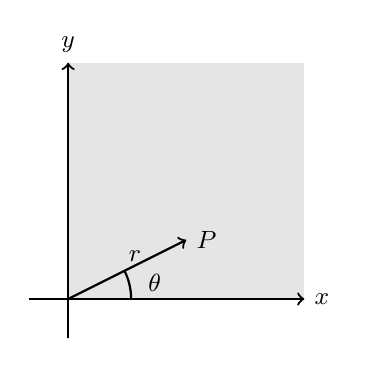
\begin{tikzpicture}[scale=1]
            % Sombreado leve en todo el primer cuadrante
            \fill[black,opacity=0.1] (0,0) -- (3,0) -- (3,3) -- (0,3) -- cycle;

            % Ejes
            \draw[thick,->] (-0.5,0) -- (3,0) node[right] {\small $x$};
            \draw[thick,->] (0,-0.5) -- (0,3) node[above] {\small $y$};

            % Vector r con "r" más arriba y "P" en la punta
            \draw[thick,->] (0,0) -- (1.5,0.75) node[right] {\small $P$};
            \node at (0.85,0.55) {\small $r$};  % "r" más arriba en la flecha

            % Ángulo theta
            \draw[thick] (0.8,0) arc (0:26.57:0.8);
            \node at (1.1,0.2) {\small $\theta$};
        \end{tikzpicture}
    \end{center}

    Así finalmente la integral da
    \[
        \frac{1}{2} \text{area}(E) = \frac{1}{2} \cdot (9-1) \cdot (8-4) = 16
    \]
}

\ejemplo{
Calcúlese el volumen comprendido entre $z = f(x,y)$, $z = g(xy)$ sobre D, con D la proyección de las funciones sobre el plano z. Entonces,
$$ vol = \int_{D}(f(x,y) - g(x,y))dx dy = \int_ {D} 1 dx dy dz = \int_{D} \left(\int_{z = g(x,y)}^{z = f(x,y)}1 dz\right)dx dy$$
    }

    \ejemplo{
    \underline{Bóveda de Viviani}\\
    Calcúlese el volumen comprendido entre la esfera $x^2 + y^2 + z^2 = a^2$ y el cilindro $x^2 + y^2 = ay$ con $a > 0$.
    \vspace{-1.2em}

    \begin{center}
        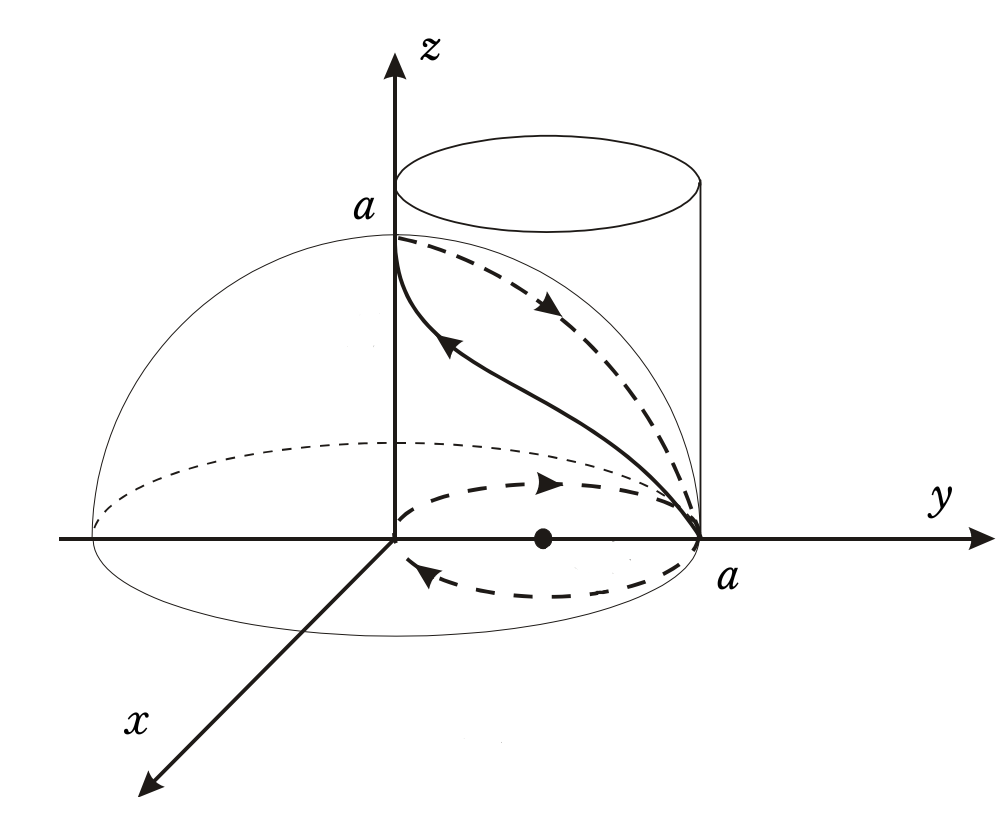
\includegraphics[width=0.4\textwidth]{images/2.png}
    \end{center}

    \vspace{-1em}

    Donde tomando valores en la esfera podemos obtener: $$\begin{cases} x^2 + y^2 - ay = 0 \iff x^2 + (y - \frac{a}{2})^2 = \frac{a^2}{4} \\ x^2 + (y - \frac{a}{2})^2 = x^2 + y^2 + \frac{a^2}{4} - ay = \frac{a^2}{4} \end{cases}$$
    Si tomamos que $r^2 = x^2 + y^2$ y $ay = ar\sin(\theta)$ entonces,
    La ecuación de la circunferencia es en coordenadas polares es: $r = a\cos(\theta)$

$$vol = 2\int_{D}\sqrt{a^2 - x^2 - y^2} dx dy = 2\int_{\theta = 0}^{\theta = 2\pi}\int_{r = 0}^{r = a\sin(\theta)}\sqrt{a^2 -r^2}r dr d\theta$$
$$ = 2\int_{\theta = 0}^{\theta = \pi} \left[-\frac{1}{3}(a^2-r^2)^{\frac{3}{2}}\right]^{r = a\sin(\theta)}_{r = 0} d\theta = \frac{2}{3} \int_{\theta = 0}^{\theta = \pi} a^3 - (a^2 - a^2\sin^2(\theta))^{\frac{3}{2}}d\theta$$
$$= \frac{2}{3}\int_{\theta = 0}^{\theta = \pi} a^3 - a^3|\cos^3(\theta)|d\theta = 4 \frac{a^3}{3}\int_{\theta=0}^{\theta = \frac{\pi}{2}} 1- \cos^3(\theta)d\theta $$
$$= \frac{4 a^3}{3} \left[\theta - \left(\sin(\theta)-\frac{\sin^3(\theta)}{3}\right) \right]_{\theta = 0}^{\theta = \frac{\pi}{2}} =  \frac{4 a^3}{3} \left(\frac{\pi}{2} - \frac{2}{3}\right) $$

Todo esto teniendo en cuenta que $(\cos^3(\theta))^{\frac{3}{2}} =
    |\cos^3(\theta)|$ }

